% Wheeled Humanoid - Design Book.
% Compile:  tectonic main.tex   (or pdflatex main.tex twice)
% Figures from the model:  .venv/bin/python designbook_latex/make_figures.py  (from the repository root)
\documentclass[11pt,a4paper]{article}
\usepackage[T1]{fontenc}
\usepackage[utf8]{inputenc}
\usepackage[scaled=0.95]{helvet}
\renewcommand{\familydefault}{\sfdefault}
\usepackage[a4paper,margin=20mm,top=24mm,bottom=24mm]{geometry}
\usepackage{graphicx,xcolor,booktabs,tabularx,longtable,array,float,caption,enumitem,amsmath,textcomp}
\usepackage{titlesec,fancyhdr,microtype,pdflscape}
\usepackage{tikz}
\usetikzlibrary{positioning,arrows.meta,fit,calc}
\usepackage[most]{tcolorbox}
\usepackage[hidelinks]{hyperref}
\usepackage{xurl}
\usepackage{needspace}

% ---------- draft switch: \drafttrue shows the "to complete" marks and the checklist page ----------
\newif\ifdraft
\draftfalse
% \draftfalse   % uncomment for the version you submit, once every mark is filled

% Black and white. The wiring sheets and the data plots keep their colours, which carry information
% (wire function, one colour per signal).
\definecolor{rule}{gray}{0.0}
\definecolor{soft}{gray}{0.95}
\definecolor{pwr}{HTML}{C0392B}\definecolor{sig}{HTML}{2C6FBB}\definecolor{sda}{HTML}{1E8E4E}
\definecolor{scl}{HTML}{D9820B}\definecolor{act}{HTML}{E08E0B}

\newcommand{\todo}[1]{\ifdraft\textbf{[TO COMPLETE: #1]}\else #1\fi}
\newcommand{\kgcm}{kg\textperiodcentered cm}
\newcommand{\file}[1]{{\small\nolinkurl{#1}}}
\renewcommand{\deg}{\textdegree}
\newcommand{\repo}{https://github.com/Cymric-tn/wheeled-humanoid}

\titleformat{\section}{\Large\bfseries}{\thesection}{0.6em}{}[\vspace{-4pt}\rule{\linewidth}{0.5pt}]
\titleformat{\subsection}{\large\bfseries}{\thesubsection}{0.6em}{}
\titleformat{\subsubsection}{\normalsize\bfseries}{\thesubsubsection}{0.6em}{}
\titlespacing*{\section}{0pt}{14pt}{8pt}
\titlespacing*{\subsection}{0pt}{10pt}{4pt}
\setlist{nosep,leftmargin=1.4em}
\setlength{\parindent}{0pt}\setlength{\parskip}{5pt}
\captionsetup{font=small,labelfont=bf}
\renewcommand{\arraystretch}{1.18}
\pagestyle{fancy}\fancyhf{}
\lhead{\small RAS Build Challenge \textperiodcentered{} Project 2 \textperiodcentered{} Wheeled Humanoid}
\rhead{\small Design Book}
\cfoot{\small\thepage}
\renewcommand{\headrulewidth}{0.4pt}
\newtcolorbox{keybox}[1][]{colback=white,colframe=black,boxrule=0.5pt,arc=0pt,left=6pt,right=6pt,top=4pt,bottom=4pt,#1}
\newcolumntype{L}{>{\raggedright\arraybackslash}X}
\newcolumntype{P}[1]{>{\raggedright\arraybackslash}p{#1}}

\begin{document}

% =============================================================== title
\begin{titlepage}
\centering
{\small\bfseries RAS BUILD CHALLENGE \textperiodcentered{} DESIGN PHASE \textperiodcentered{} PROJECT 2}\par\vspace{10mm}
{\fontsize{36}{42}\selectfont\bfseries Wheeled Humanoid}\par\vspace{4mm}
{\LARGE Design Book}\par\vspace{5mm}
\rule{\linewidth}{0.8pt}\par\vspace{2mm}
{\normalsize IEEE RAS Tunisia Section $\times$ ODC FabLab \textperiodcentered{} submission of 16 November 2026}\par
\vfill
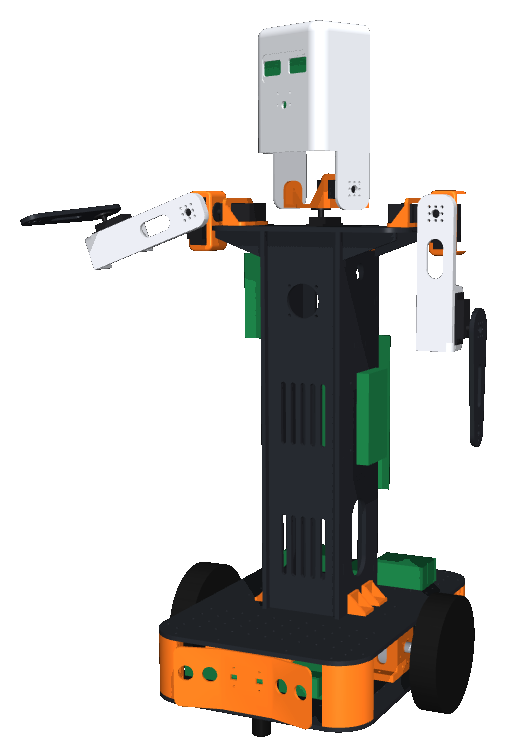
\includegraphics[height=170mm]{figs/v2_cover.png}\par
\vfill
\end{titlepage}

% =============================================================== checklist (draft only)
\ifdraft
\section*{Before you submit (this page disappears with \texttt{\textbackslash draftfalse})}
Items marked \textbf{[TO COMPLETE]} through the document still need the team:
\begin{enumerate}
\item \textbf{Sheet material} for the laser-cut plates is not fixed yet. The book uses acrylic (4.79\,kg robot) and gives plywood (3.87\,kg) alongside; once the FabLab confirms, only the masses change.
\item \textbf{Send the part requests} of section~\ref{sec:bom} to \texttt{ras@ieee.tn}; the spec book asks for them early.
\item Every dimension of a kit part is a typical value until the kit is in hand (21~November). This is stated in section~\ref{sec:cad} and is not something to hide.
\end{enumerate}
\clearpage
\fi

\setcounter{tocdepth}{2}
\tableofcontents

\clearpage

% =============================================================== 1 technical study
\section{Technical study}\label{sec:study}

\subsection{Mission, requirements and success criteria}
The robot must drive on its wheels, stop before an obstacle, and give the upper body its character with one arm movement and one head gesture. The design targets the minimum demonstration first; everything else is optional and independent.

\begin{table}[H]\small
\begin{tabularx}{\linewidth}{@{}P{9mm}P{50mm}LP{38mm}@{}}
\toprule
\textbf{ID} & \textbf{Requirement (spec book)} & \textbf{How the design meets it} & \textbf{Success criterion}\\
\midrule
R1 & Drive forward and backward, turn on the spot, using the wheel encoders & Two encoder gearmotors; each wheel tracks a position reference with a speed loop; turns measured in encoder counts and cross-checked with the gyro & 2\,m: error under 5\,cm. 90\deg: error under 5\deg\\
R2 & Detect an obstacle in front and stop at a safe distance & Two VL53L0X and two HC-SR04 on the front bar; braking starts at 55\,cm & Stops between 30 and 40\,cm, never touches\\
R3 & Perform an arm movement & Two 3-DOF arms (shoulder pitch, shoulder roll, elbow), interpolated motion & 20 waves with no stall and no controller reset\\
R4 & Perform a head gesture & Pan and tilt head & 20 nods, smooth\\
R5 & Minimum demonstration: move, turn, stop before an obstacle, arm movement, head gesture & One stored sequence on the Mega, started by one command (\texttt{DEMO}) & 5 runs out of 5 with no intervention\\
R6 & Only the provided hardware; additions must not affect the timeline & Every kit part is used and placed (section~\ref{sec:bom}); ten small requests & Minimum demonstration works without any optional part\\
\bottomrule
\end{tabularx}
\end{table}

\subsection{System architecture}
\subsubsection{Mechanical block diagram}
\begin{figure}[H]\centering
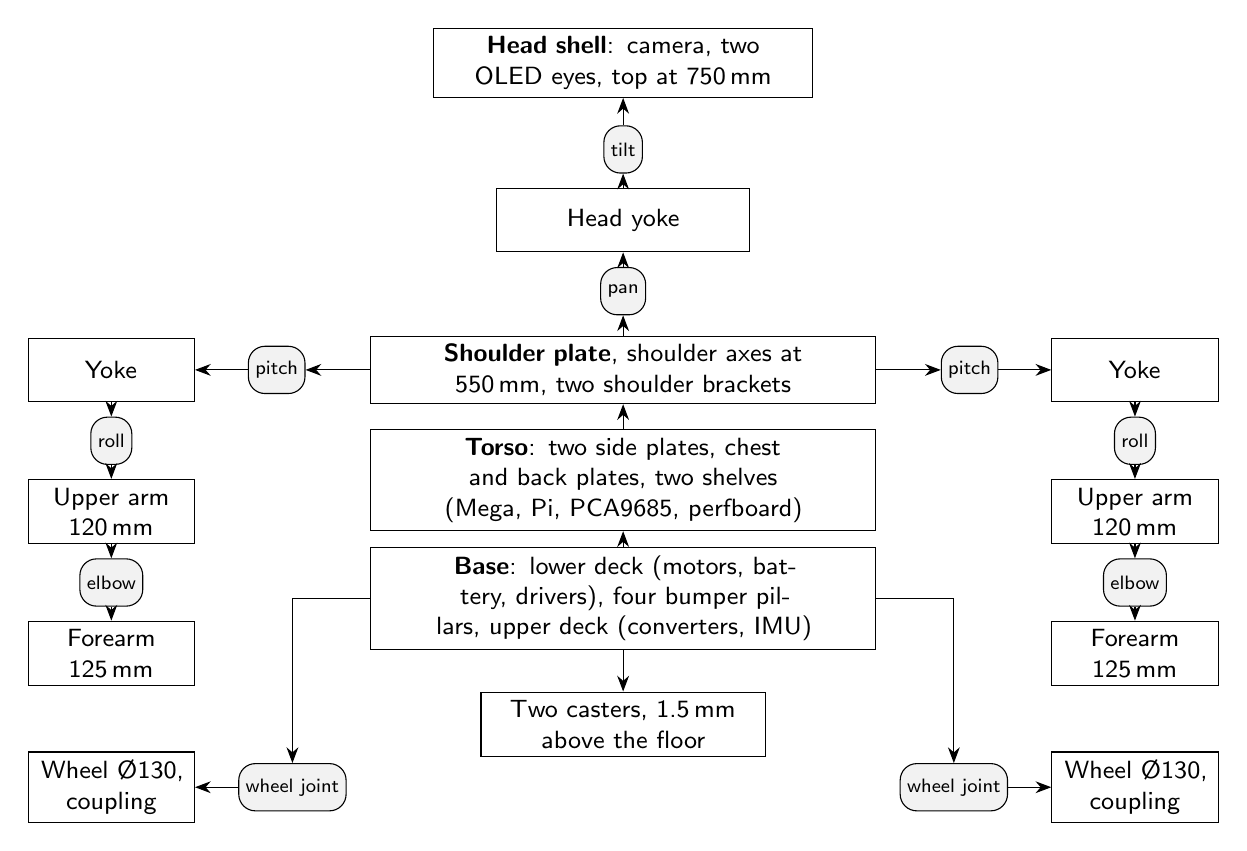
\begin{tikzpicture}[font=\small,
  blk/.style={draw=black,fill=white,minimum height=8mm,align=center,inner sep=3pt},
  jnt/.style={draw=black,rounded corners=6pt,fill=soft,minimum height=6mm,align=center,inner sep=2.5pt,font=\scriptsize},
  >={Stealth[length=2mm]}]
\node[blk,text width=46mm] (head) at (0,6.7) {\textbf{Head shell}: camera, two OLED eyes, top at 750\,mm};
\node[jnt] (tilt) at (0,5.6) {tilt};
\node[blk,text width=30mm] (hy) at (0,4.7) {Head yoke};
\node[jnt] (pan) at (0,3.8) {pan};
\node[blk,text width=62mm] (sh) at (0,2.8) {\textbf{Shoulder plate}, shoulder axes at 550\,mm, two shoulder brackets};
\node[blk,text width=62mm] (torso) at (0,1.4) {\textbf{Torso}: two side plates, chest and back plates, two shelves (Mega, Pi, PCA9685, perfboard)};
\node[blk,text width=62mm] (base) at (0,-0.1) {\textbf{Base}: lower deck (motors, battery, drivers), four bumper pillars, upper deck (converters, IMU)};
\node[blk,text width=34mm] (cas) at (0,-1.7) {Two casters, 1.5\,mm above the floor};
\foreach \s/\n in {-1/l,1/r}{
  \node[jnt] (\n p) at (\s*4.4,2.8) {pitch};
  \node[blk,text width=19mm] (\n y) at (\s*6.5,2.8) {Yoke};
  \node[jnt] (\n r) at (\s*6.5,1.9) {roll};
  \node[blk,text width=19mm] (\n u) at (\s*6.5,1.0) {Upper arm 120\,mm};
  \node[jnt] (\n e) at (\s*6.5,0.1) {elbow};
  \node[blk,text width=19mm] (\n f) at (\s*6.5,-0.8) {Forearm 125\,mm};
  \node[jnt] (\n w) at (\s*4.2,-2.5) {wheel joint};
  \node[blk,text width=19mm] (\n wh) at (\s*6.5,-2.5) {Wheel \O130, coupling};
  \draw[->] (sh)--(\n p); \draw[->] (\n p)--(\n y); \draw[->] (\n y)--(\n r); \draw[->] (\n r)--(\n u); \draw[->] (\n u)--(\n e); \draw[->] (\n e)--(\n f);
  \draw[->] (base) -| (\n w); \draw[->] (\n w) -- (\n w -| \n wh.\ifnum\s<0 east\else west\fi);
}
\draw[->] (base)--(torso); \draw[->] (torso)--(sh); \draw[->] (base)--(cas);
\draw[->] (sh)--(pan); \draw[->] (pan)--(hy); \draw[->] (hy)--(tilt); \draw[->] (tilt)--(head);
\end{tikzpicture}
\caption{Mechanical structure. Square boxes are rigid bodies, rounded grey boxes the ten actuated joints (two wheels, six arm joints, two head joints).}
\end{figure}

\subsubsection{Electronic block diagram}
\begin{figure}[H]\centering
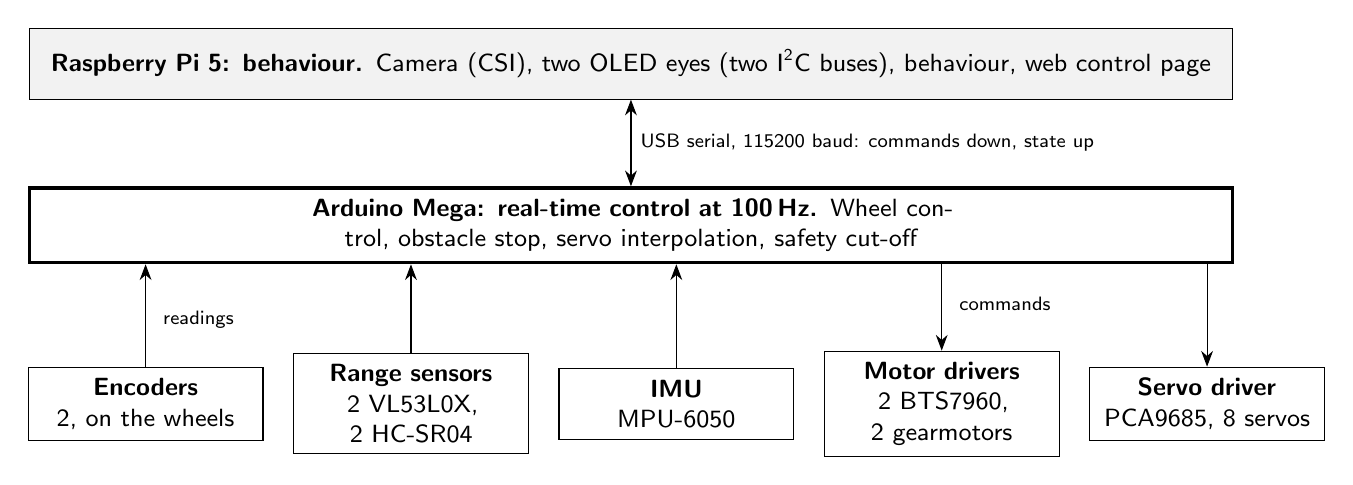
\begin{tikzpicture}[font=\small,
  blk/.style={draw=black,minimum height=9mm,align=center,inner sep=4pt,text width=27mm,fill=white},
  >={Stealth[length=2mm]}]
\node[blk,text width=150mm,fill=soft] (pi) {\textbf{Raspberry Pi 5: behaviour.} Camera (CSI), two OLED eyes (two I\textsuperscript{2}C buses), behaviour, web control page};
\node[blk,text width=150mm,line width=1.2pt,below=11mm of pi] (mega) {\textbf{Arduino Mega: real-time control at 100\,Hz.} Wheel control, obstacle stop, servo interpolation, safety cut-off};
\draw[<->] (pi)--node[right,font=\scriptsize]{USB serial, 115200 baud: commands down, state up} (mega);
\node[blk,below=13mm of mega.south west,anchor=north west] (enc) {\textbf{Encoders}\\2, on the wheels};
\node[blk,right=3.75mm of enc] (rng) {\textbf{Range sensors}\\2 VL53L0X, 2 HC-SR04};
\node[blk,right=3.75mm of rng] (imu) {\textbf{IMU}\\MPU-6050};
\node[blk,right=3.75mm of imu] (mot) {\textbf{Motor drivers}\\2 BTS7960, 2 gearmotors};
\node[blk,right=3.75mm of mot] (srv) {\textbf{Servo driver}\\PCA9685, 8 servos};
\foreach \n in {enc,rng,imu} \draw[->] (\n.north)--(\n.north |- mega.south);
\foreach \n in {mot,srv} \draw[->] (\n.north |- mega.south)--(\n.north);
\node[font=\scriptsize,anchor=west] at ($(enc.north)+(1mm,6mm)$) {readings};
\node[font=\scriptsize,anchor=west] at ($(mot.north)+(1mm,6mm)$) {commands};
\end{tikzpicture}
\caption{Control is split in two layers. The Mega reads every sensor and drives every actuator; the Pi only sends short text commands.}
\end{figure}

\subsubsection{Software block diagram}
\begin{figure}[H]\centering
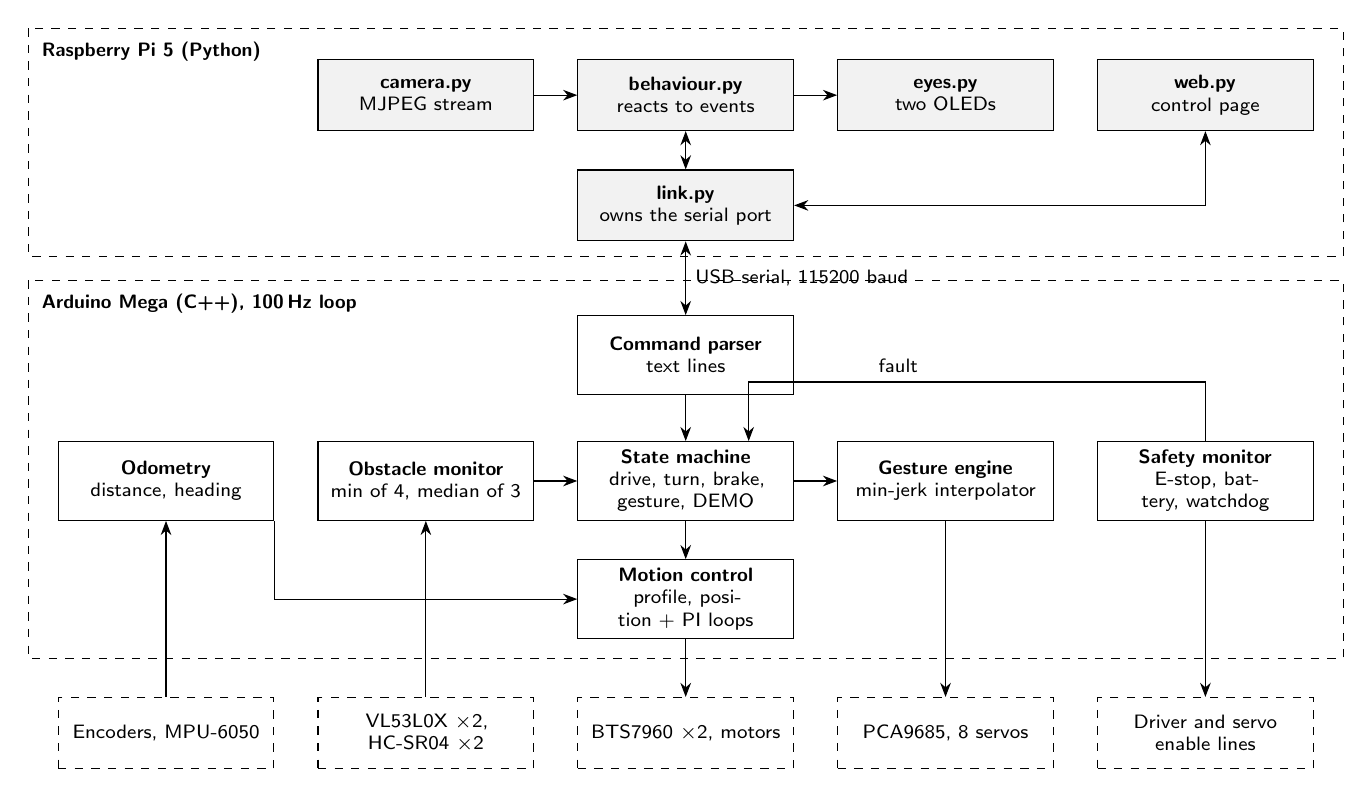
\begin{tikzpicture}[font=\scriptsize,
  m/.style={draw=black,fill=white,minimum height=10mm,align=center,text width=26mm,inner sep=2pt},
  p/.style={draw=black,fill=soft,minimum height=9mm,align=center,text width=26mm,inner sep=2pt},
  h/.style={draw=black,dashed,minimum height=9mm,align=center,text width=26mm,inner sep=2pt,fill=white},
  >={Stealth[length=1.8mm]}]
\draw[dashed] (-1.75,0.85) rectangle (14.95,-2.05);
\draw[dashed] (-1.75,-2.35) rectangle (14.95,-7.15);
\node[anchor=north west,font=\scriptsize\bfseries] at (-1.7,0.8) {Raspberry Pi 5 (Python)};
\node[anchor=north west,font=\scriptsize\bfseries] at (-1.7,-2.4) {Arduino Mega (C++), 100\,Hz loop};
\node[p] (cam) at (3.3,0) {\textbf{camera.py}\\MJPEG stream};
\node[p] (beh) at (6.6,0) {\textbf{behaviour.py}\\reacts to events};
\node[p] (eyes) at (9.9,0) {\textbf{eyes.py}\\two OLEDs};
\node[p] (web) at (13.2,0) {\textbf{web.py}\\control page};
\node[p] (link) at (6.6,-1.4) {\textbf{link.py}\\owns the serial port};
\node[m] (par) at (6.6,-3.3) {\textbf{Command parser}\\text lines};
\node[m] (odo) at (0,-4.9) {\textbf{Odometry}\\distance, heading};
\node[m] (obs) at (3.3,-4.9) {\textbf{Obstacle monitor}\\min of 4, median of 3};
\node[m] (fsm) at (6.6,-4.9) {\textbf{State machine}\\drive, turn, brake, gesture, DEMO};
\node[m] (ges) at (9.9,-4.9) {\textbf{Gesture engine}\\min-jerk interpolator};
\node[m] (saf) at (13.2,-4.9) {\textbf{Safety monitor}\\E-stop, battery, watchdog};
\node[m] (mot) at (6.6,-6.4) {\textbf{Motion control}\\profile, position + PI loops};
\node[h] (enc) at (0,-8.1) {Encoders, MPU-6050};
\node[h] (rng) at (3.3,-8.1) {VL53L0X $\times$2, HC-SR04 $\times$2};
\node[h] (bts) at (6.6,-8.1) {BTS7960 $\times$2, motors};
\node[h] (pca) at (9.9,-8.1) {PCA9685, 8 servos};
\node[h] (en) at (13.2,-8.1) {Driver and servo enable lines};
\draw[->] (cam)--(beh); \draw[->] (beh)--(eyes); \draw[<->] (beh)--(link); \draw[<->] (web) |- (link);
\draw[<->] (link)--node[right]{USB serial, 115200 baud} (par);
\draw[->] (par)--(fsm); \draw[->] (obs)--(fsm); \draw[->] (fsm)--(ges); \draw[->] (fsm)--(mot);
\draw[->] (saf.north) |- ++(-2.0,0.75) -| node[pos=0.25,above]{fault} ([xshift=8mm]fsm.north);
\draw[->] (enc)--(odo); \draw[->] (rng)--(obs); \draw[->] (mot)--(bts); \draw[->] (ges)--(pca); \draw[->] (saf)--(en);
\draw[->] (odo.south east) |- (mot.west);
\end{tikzpicture}
\caption{Software modules. Grey: Python on the Pi. White: firmware on the Mega. Dashed: hardware.}
\end{figure}

\subsection{Design choices and their justification}
\begin{table}[H]\small
\begin{tabularx}{\linewidth}{@{}P{33mm}P{45mm}L@{}}
\toprule
\textbf{Topic} & \textbf{Choice} & \textbf{Why, and what was rejected}\\
\midrule
Controller split & Mega does all real-time work; Pi only sends commands & The minimum demonstration cannot depend on a Linux boot, an SD card or a camera stack. Rejected: Pi driving the PCA9685 and motors directly, which makes every gesture depend on the Pi.\\
Base & Two decks, drive wheels on the centre axis, one caster in front and one behind & Turns on the spot about its own centre; the lower deck carries the heavy parts 35 to 120\,mm above the floor. Rejected: a single deck, which puts converters and drivers higher and raises the centre of mass.\\
Caster height & Casters 1.5\,mm above the floor & With four contact points a drive wheel can lift on an uneven floor and corrupt the odometry. With the casters raised, both drive wheels always carry load.\\
Battery position & 95\,mm behind the wheel axis & Puts the centre of mass 6.5\,mm behind the axle, so the robot rests on its rear caster in a defined three-point stance (section~\ref{sec:stab}).\\
Wheel control & Each wheel tracks a position reference, speed capped at 0.40\,m/s, acceleration at 0.5\,m/s\textsuperscript{2} & Tracking position, not only speed, makes the robot stop on target despite motor lag (found in simulation, section~\ref{sec:sim}). 29\,\% of the motor's speed and 25\,\% of its force: safe indoors, short braking distance, tip-over margin of 13.\\
Arm layout & Pitch, then roll, then elbow; the 30\,\kgcm{} servos on the two shoulder axes & The shoulder axes carry the whole arm; the 18\,\kgcm{} servo only carries the forearm. Each servo body sits in the link before its joint, so no servo is carried further out than necessary.\\
Servo power & Two 6.8\,V rails, one per arm, fed directly from the converters to a header strip & The PCA9685 power traces are not sized for stalled 30\,\kgcm{} servos. Splitting by arm halves the peak on each converter. 6.8\,V is within the limit of the MG996.\\
Emergency stop & Cuts actuators only & The Pi and Mega stay powered, report the state and restart cleanly. Rejected: cutting the battery, which hard-powers-off the Pi.\\
Obstacle sensing & Two sensor types, minimum of all four & ToF is precise but narrow and fails on dark or glossy surfaces; ultrasonic is wide but coarse. Each covers the other's blind case.\\
Servo motion & Minimum-jerk interpolation, peak 90\deg/s & No servo is ever commanded to jump: lower current peaks, no shaking of a 75\,cm structure, and the motion reads as intentional.\\
Structure material & 5\,mm laser-cut sheet for the 11 plates, PLA prints for every servo and motor interface & Plates are fast and stiff; print time goes only where 3D shape is needed (about 550\,g of filament in total).\\
Pi software & Plain Python on Raspberry Pi OS, no ROS & One robot, no lidar, no navigation stack: ROS would add setup time and nothing the demonstration needs. The serial protocol leaves the door open to wrap it in a ROS~2 node later.\\
\bottomrule
\end{tabularx}
\end{table}

\subsection{Calculations}
Masses come from the CAD: part volume times material density (5\,mm acrylic 1190\,kg/m\textsuperscript{3}; PLA prints at an effective 750\,kg/m\textsuperscript{3} for 30 to 40\,\% infill with walls) plus a typical mass for each kit component at its placed position. They are computed by the digital twin (\file{sim/generate_twin.py}) and will be replaced by weighed values when the kit is received. With plywood plates (680\,kg/m\textsuperscript{3}) the robot is 0.92\,kg lighter.

\subsubsection{Mass and stability}\label{sec:stab}
\begin{table}[H]\small
\begin{tabularx}{\linewidth}{@{}LP{30mm}L@{}}
\toprule
\textbf{Quantity} & \textbf{Value} & \textbf{Basis}\\
\midrule
Total mass & 4.79\,kg & Twin, acrylic plates (3.87\,kg with plywood)\\
Centre of mass height & 217\,mm & 29\,\% of the 750\,mm height\\
Centre of mass, fore-aft & 6.5\,mm behind the axle & Battery and converters at the rear\\
Support distance (worst case) & 143.5\,mm & Centre of mass to the rear caster (casters at $\pm$150\,mm)\\
Static tip angle & 33.5\deg & $\arctan(143.5/217)$\\
Acceleration that tips the robot & 6.5\,m/s\textsuperscript{2} & $g \times 143.5/217$; the firmware limit is 0.5\,m/s\textsuperscript{2}, a factor of 13\\
Braking that stays on the rear caster & below 0.29\,m/s\textsuperscript{2} & $a < g\,x/h = 9.81 \times 6.5/217$\\
\bottomrule
\end{tabularx}
\end{table}
\textbf{Consequence.} At the 0.5\,m/s\textsuperscript{2} braking limit the robot rocks forward onto its front caster, a 1.5\,mm drop or 0.6\deg. The simulation shows exactly this (maximum body tilt 0.64\deg, section~\ref{sec:sim}): harmless, and far from tipping. If it disturbs the head camera, the battery moves 6\,mm further back or the braking limit drops to 0.3\,m/s\textsuperscript{2}.

\subsubsection{Kinematics and speed}
\textbf{Differential drive.} With wheel radius $R = 65$\,mm, wheel track $W = 300$\,mm and wheel speeds $\omega_L$, $\omega_R$:
\[ v = \frac{R(\omega_R+\omega_L)}{2}, \qquad \dot\theta = \frac{R(\omega_R-\omega_L)}{W}, \qquad
\omega_{L,R} = \frac{v \mp \dot\theta\,W/2}{R}. \]
Odometry integrates the wheel travels $s_L$, $s_R$ read from the encoders: distance $d=(s_R+s_L)/2$, heading $\theta=(s_R-s_L)/W$. One encoder count is $2\pi R/N = 408.4/N$\,mm of travel, where $N$ is the counts per wheel revolution (assumption: $N = 1320$, from 11 pulses per motor turn, a 30:1 gearbox and 4 edges, typical for 12\,V 200\,rpm encoder gearmotors; one count is then 0.31\,mm). A 90\deg{} turn on the spot is $W\pi/4 = 235.6$\,mm of travel on each wheel, in opposite directions.

\begin{table}[H]\small
\begin{tabularx}{\linewidth}{@{}LP{28mm}L@{}}
\toprule
\textbf{Quantity} & \textbf{Value} & \textbf{Basis}\\
\midrule
Top speed at 100\,\% PWM & 1.36\,m/s & 200\,rpm on $R=65$\,mm\\
Speed cap in firmware & 0.40\,m/s & 59\,rpm, about 29\,\% PWM\\
Acceleration and braking limit & 0.5\,m/s\textsuperscript{2} & Ramp limiter on the speed reference\\
Turn rate & 0.8\,rad/s & Wheel speeds $\pm$0.12\,m/s; 90\deg{} in about 2.5\,s\\
Theoretical braking distance & 16\,cm & $v^2/2a$; 15.0\,cm measured in the twin (section~\ref{sec:sim})\\
\bottomrule
\end{tabularx}
\end{table}

\textbf{Arm.} Each arm has shoulder pitch $\theta_1$ (about the lateral axis), shoulder roll $\theta_2$ (about the forward axis) and elbow $\theta_3$, with $L_1 = 120$\,mm from shoulder to elbow and $L_2 = 125$\,mm from elbow to fingertip. In the shoulder frame ($x$ forward, $z$ up, all angles zero with the arm hanging), the fingertip is at
\[ \mathbf{p} = R_y(-\theta_1)\,R_x(\pm\theta_2)\left[\begin{pmatrix}0\\0\\-L_1\end{pmatrix} + R_y(-\theta_3)\begin{pmatrix}0\\0\\-L_2\end{pmatrix}\right], \]
which for $\theta_2=0$ reduces to $x = L_1\sin\theta_1 + L_2\sin(\theta_1+\theta_3)$, $z = -L_1\cos\theta_1 - L_2\cos(\theta_1+\theta_3)$. The reach is 245\,mm: with the shoulder axis at 550\,mm the fingertip is at 305\,mm when the arm hangs, 245\,mm ahead of the shoulder when pointing, and at 795\,mm when raised. Gestures are defined in joint space (keyframes of $\theta_1,\theta_2,\theta_3$), so no inverse kinematics is needed for the demonstration.

\subsubsection{Torque and load}
\begin{table}[H]\small
\begin{tabularx}{\linewidth}{@{}P{42mm}P{24mm}P{22mm}P{20mm}L@{}}
\toprule
\textbf{Actuator} & \textbf{Load} & \textbf{Rated} & \textbf{Share} & \textbf{Case}\\
\midrule
Drive, both motors & 7.7\,N & 30.2\,N & 25\,\% & Accelerating at 0.5\,m/s\textsuperscript{2} (2.4\,N) on a 5\deg{} ramp (4.1\,N) with rolling resistance (1.2\,N)\\
Shoulder pitch, TD-8130MG & 1.4\,\kgcm & 30\,\kgcm & 5\,\% & Arm horizontal forward, static\\
Shoulder pitch with 100\,g in the hand & 3.8\,\kgcm & 30\,\kgcm & 13\,\% & Payload at 245\,mm\\
Shoulder roll, TD-8130MG & 1.3\,\kgcm & 30\,\kgcm & 4\,\% & Arm horizontal sideways, static\\
Elbow, RCXAZ & 0.13\,\kgcm & 18\,\kgcm & under 1\,\% & Forearm horizontal\\
Head tilt, MG996 & 0.8\,\kgcm & 13\,\kgcm & 6\,\% & Head tilted 30\deg\\
\bottomrule
\end{tabularx}
\end{table}
The static torques are computed by the twin at each pose (gravity term of the joint). The moving arm weighs 180\,g with its centre of mass 75\,mm from the shoulder pitch axis. The design rule is that no joint exceeds a third of its rated torque, including the dynamic peaks measured in simulation (section~\ref{sec:sim}). Assumption: the motor's 10\,\kgcm{} is taken as its stall torque, with 5\,A of stall current; a real stall torque above the rated value only adds margin.

\subsubsection{Power budget and battery life}
\begin{table}[H]\small
\begin{tabularx}{\linewidth}{@{}P{52mm}P{22mm}P{20mm}L@{}}
\toprule
\textbf{Load, current at the battery} & \textbf{Typical} & \textbf{Peak} & \textbf{Basis}\\
\midrule
Two drive motors & 2.0\,A & 10.0\,A & 1\,A each cruising, 5\,A each assumed at stall\\
Eight servos through two converters & 1.4\,A & 8.2\,A & Each converter limited to about 6\,A output at 6.8\,V\\
Raspberry Pi 5 with camera & 0.5\,A & 1.2\,A & 5\,W typical, 12\,W peak\\
Mega, sensors, OLEDs & 0.15\,A & 0.2\,A & About 1.5\,W\\
\midrule
\textbf{Total} & \textbf{4.05\,A} & \textbf{19.6\,A} & Peak stays under the 20\,A fuse\\
\bottomrule
\end{tabularx}
\end{table}
\textbf{Battery life:} $5.2\,\text{Ah} \times 80\,\%$ usable $/\,4.05$\,A is about 60 minutes of continuous operation. Cut-off at 9.9\,V (3.3\,V per cell), enforced by the firmware. The currents are estimates to be replaced by bench measurements.

\subsection{Wiring diagram}\label{sec:wiring}
The wiring is drawn at terminal level on three sheets (power, signals, servos) that follow on landscape pages, then the tables to wire from. Source and PDF: \file{wiring/wheeled_humanoid_wiring.drawio} and \file{.pdf} in the repository. The wire colours on the sheets carry meaning (red power, black ground, one colour per signal type) and are kept.

\begin{landscape}
\begin{figure}[p]\centering\special{pdf:put @thispage <</Rotate 90>>}
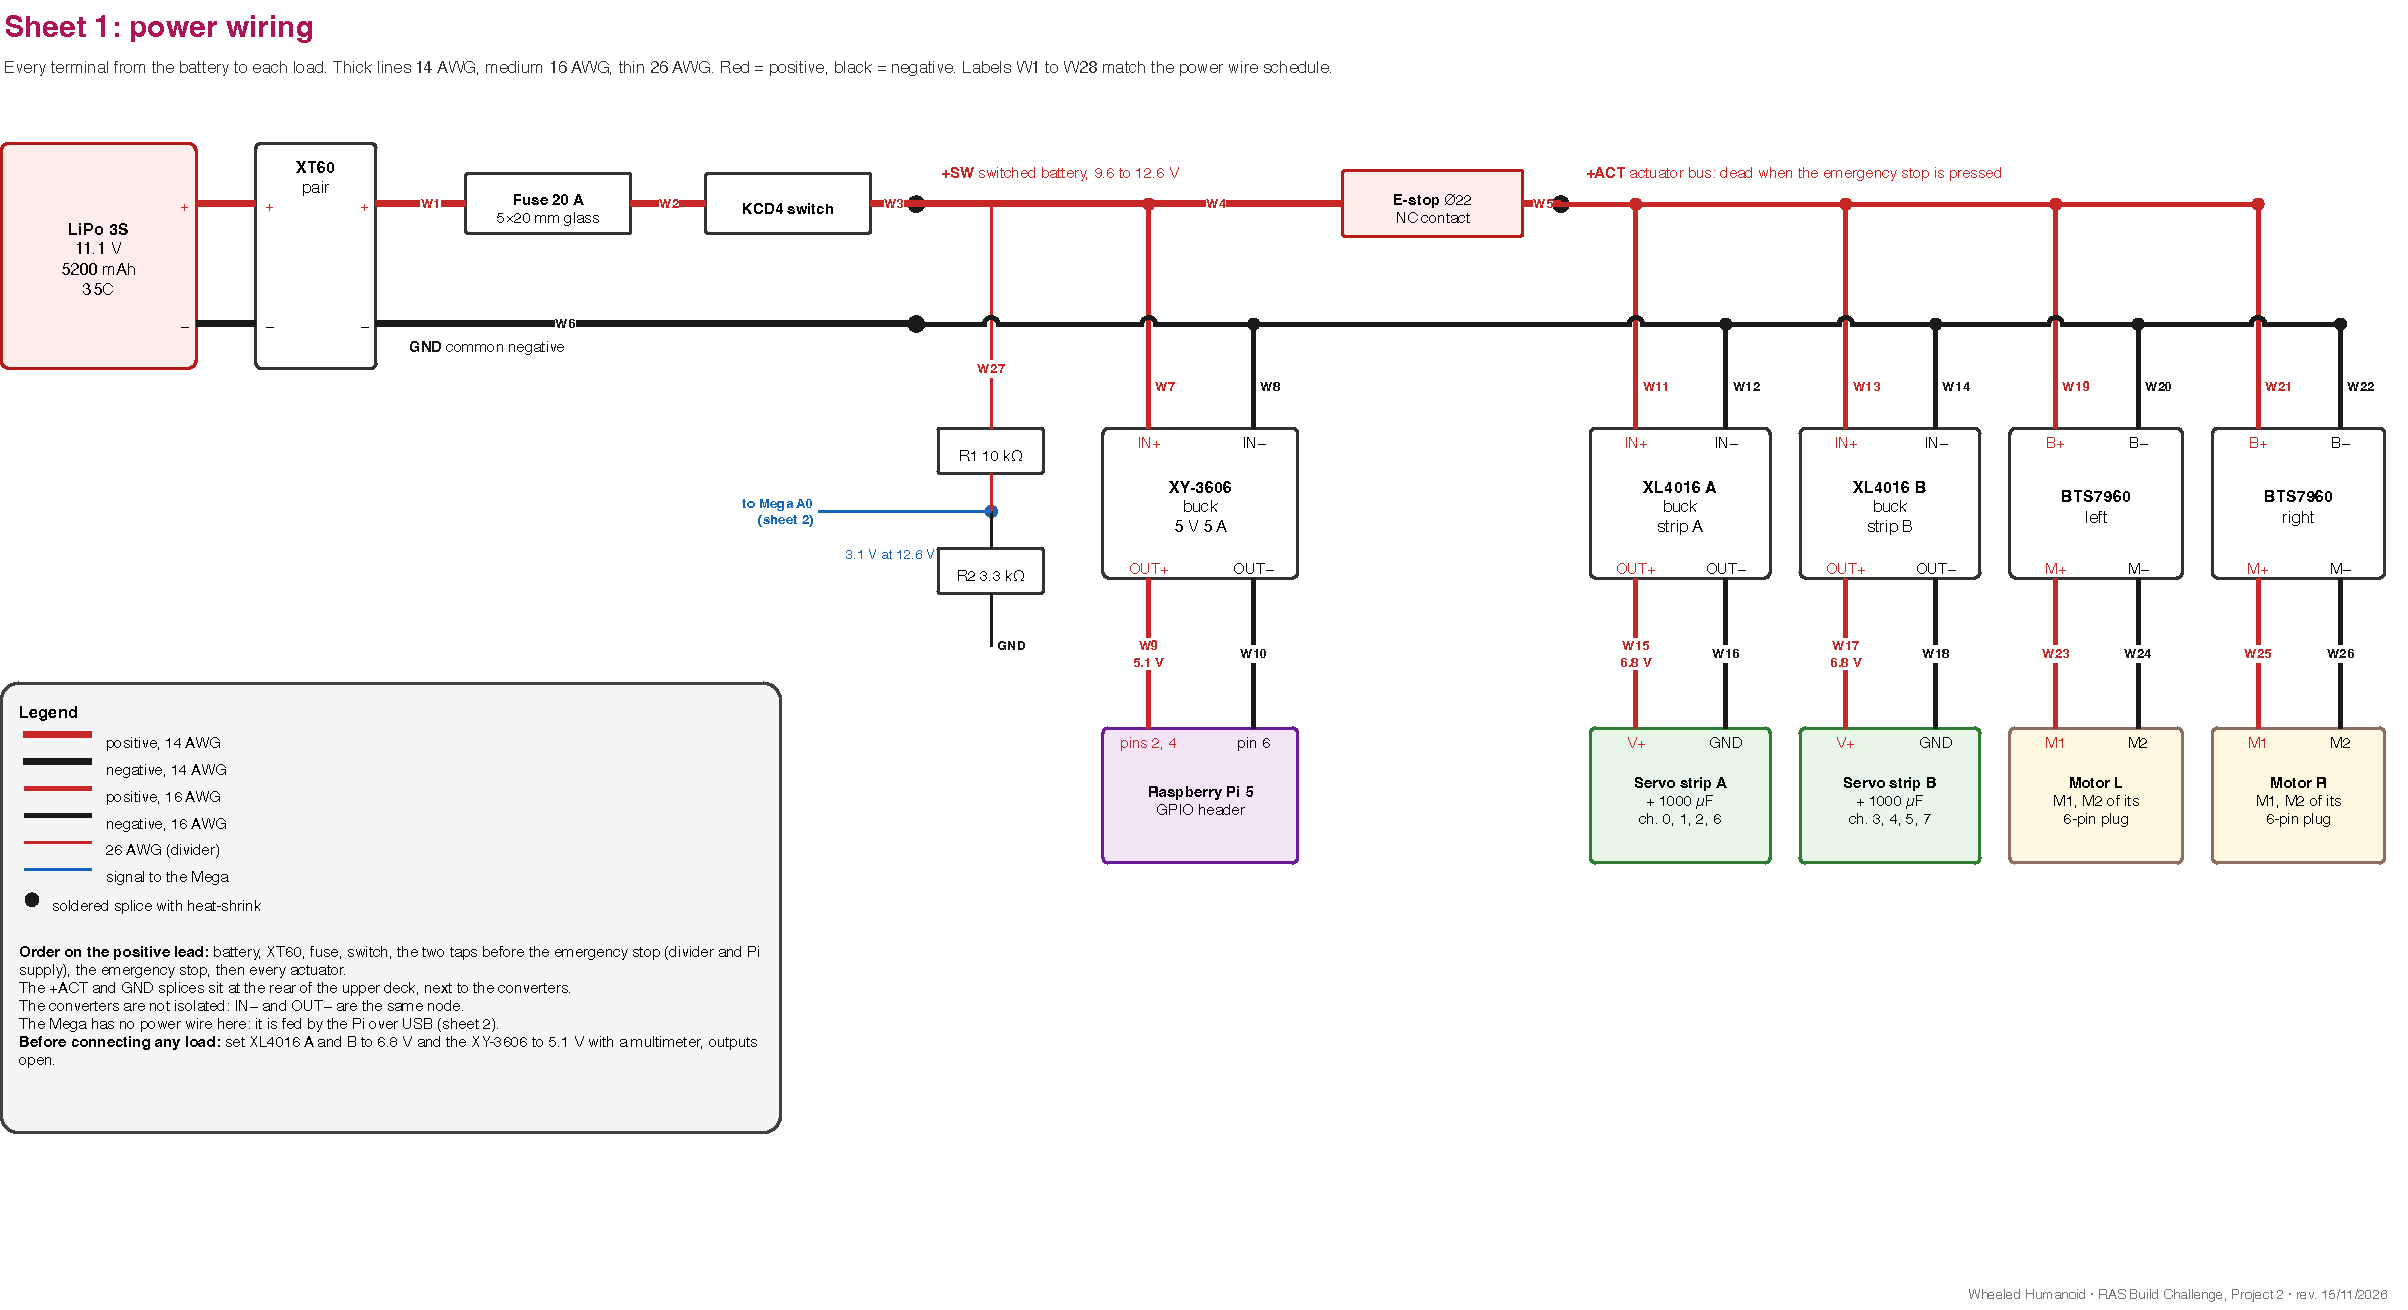
\includegraphics[width=\linewidth,height=0.9\textheight,keepaspectratio,page=1]{figs/v2_wiring.pdf}
\caption{Sheet 1, power: battery, fuse, switch, emergency stop, converters and every load. Wire numbers W1 to W28 match the wire schedule below.}\label{fig:wiring}
\end{figure}
\begin{figure}[p]\centering\special{pdf:put @thispage <</Rotate 90>>}
\includegraphics[width=\linewidth,height=0.9\textheight,keepaspectratio,page=2]{figs/v2_wiring.pdf}
\caption{Sheet 2, signals: every module pin to its Mega or Pi pin.}
\end{figure}
\begin{figure}[p]\centering\special{pdf:put @thispage <</Rotate 90>>}
\includegraphics[width=\linewidth,height=0.9\textheight,keepaspectratio,page=3]{figs/v2_wiring.pdf}
\caption{Sheet 3, servos: PCA9685 channels to the two servo strips and their 6.8\,V converters.}
\end{figure}
\end{landscape}

% ---------------------------------------------------------------- power wire schedule
\subsubsection*{Power wire schedule}
{\small
\begin{longtable}{@{}lP{41mm}P{46mm}llr@{}}
\toprule
\textbf{No.} & \textbf{From} & \textbf{To} & \textbf{Gauge} & \textbf{Colour} & \textbf{cm}\\
\midrule\endhead
W1 & Battery XT60, + & Fuse holder, in & 14 AWG & red & 15\\
W2 & Fuse holder, out & KCD4 switch, in & 14 AWG & red & 8\\
W3 & KCD4 switch, out & Splice +SW & 14 AWG & red & 5\\
W4 & Splice +SW & Emergency stop, NC in & 14 AWG & red & 8\\
W5 & Emergency stop, NC out & Splice +ACT & 14 AWG & red & 8\\
W6 & Battery XT60, $-$ & Splice GND & 14 AWG & black & 20\\
W7, W8 & Splice +SW, splice GND & XY-3606 IN+, IN$-$ & 16 AWG & red, black & 2 $\times$ 15\\
W9, W10 & XY-3606 OUT+, OUT$-$ & Pi header pins 2 and 4, pin 6 & 16 AWG & red, black & 2 $\times$ 45\\
W11, W12 & Splice +ACT, splice GND & XL4016 A IN+, IN$-$ & 16 AWG & red, black & 2 $\times$ 15\\
W13, W14 & Splice +ACT, splice GND & XL4016 B IN+, IN$-$ & 16 AWG & red, black & 2 $\times$ 15\\
W15, W16 & XL4016 A OUT+, OUT$-$ & Servo strip A, V+ and GND & 16 AWG & red, black & 2 $\times$ 35\\
W17, W18 & XL4016 B OUT+, OUT$-$ & Servo strip B, V+ and GND & 16 AWG & red, black & 2 $\times$ 35\\
W19, W20 & Splice +ACT, splice GND & BTS7960 left B+, B$-$ & 16 AWG & red, black & 2 $\times$ 35\\
W21, W22 & Splice +ACT, splice GND & BTS7960 right B+, B$-$ & 16 AWG & red, black & 2 $\times$ 35\\
W23, W24 & BTS7960 left M+, M$-$ & Left motor M1, M2 & motor cable & -- & supplied\\
W25, W26 & BTS7960 right M+, M$-$ & Right motor M1, M2 & motor cable & -- & supplied\\
W27 & Splice +SW & Divider 10\,k$\Omega$, then 3.3\,k$\Omega$ to GND & 26 AWG & red & 10\\
W28 & PCA9685 GND & Servo strip A and B GND & 26 AWG & black & 10\\
\bottomrule
\end{longtable}}
\textbf{Wire budget.} 14 AWG: 64\,cm, within the 1\,m supplied. 16 AWG: about 4.6\,m, against 1\,m supplied. Signal wire: about 27\,m of conductor, and the kit contains DuPont housings and pins but no wire. Both are added to the part requests.

\subsubsection*{Servo plugs on the strips}
Each servo plug lands on a 3-pin header on the perfboard: signal from one PCA9685 channel (signal pin only), V+ and GND from its strip.
\begin{table}[H]\small
\begin{tabularx}{\linewidth}{@{}lLlll@{}}
\toprule
\textbf{PCA9685 channel} & \textbf{Joint} & \textbf{Servo} & \textbf{Strip} & \textbf{Plug: signal / V+ / GND}\\
\midrule
0 & Left shoulder pitch & TD-8130MG & A & orange / red / brown\\
1 & Left shoulder roll & TD-8130MG & A & orange / red / brown\\
2 & Left elbow & RCXAZ 18\,kg & A & orange / red / brown\\
3 & Right shoulder pitch & TD-8130MG & B & orange / red / brown\\
4 & Right shoulder roll & TD-8130MG & B & orange / red / brown\\
5 & Right elbow & RCXAZ 18\,kg & B & orange / red / brown\\
6 & Head pan & MG996 & A & orange / red / brown\\
7 & Head tilt & MG996 & B & orange / red / brown\\
\bottomrule
\end{tabularx}
\end{table}

% ---------------------------------------------------------------- netlist
\subsubsection*{Signal connection table}
{\small
\begin{longtable}{@{}P{37mm}P{27mm}P{38mm}P{50mm}@{}}
\toprule
\textbf{Module} & \textbf{Module pin} & \textbf{Goes to} & \textbf{Note}\\
\midrule\endhead
Left motor, 6-pin plug & C1 (phase A) & Mega D2 & Interrupt pin\\
 & C2 (phase B) & Mega D18 & Interrupt pin\\
 & VCC, GND & Mega 5V, GND & Encoder supply\\
 & M1, M2 & BTS7960 left M+, M$-$ & Swap if the wheel turns backwards\\
Right motor, 6-pin plug & C1 (phase A) & Mega D3 & Interrupt pin\\
 & C2 (phase B) & Mega D19 & Interrupt pin\\
 & VCC, GND & Mega 5V, GND & \\
 & M1, M2 & BTS7960 right M+, M$-$ & \\
BTS7960 left & 1 RPWM & Mega D5 & PWM, forward\\
 & 2 LPWM & Mega D6 & PWM, reverse\\
 & 3 R\_EN and 4 L\_EN & Mega D30 & Joined at the module; low disables the driver\\
 & 5 R\_IS, 6 L\_IS & not connected & Current sense, unused\\
 & 7 VCC, 8 GND & Mega 5V, GND & Logic supply\\
BTS7960 right & 1 RPWM & Mega D7 & \\
 & 2 LPWM & Mega D8 & \\
 & 3 R\_EN and 4 L\_EN & Mega D31 & \\
 & 7 VCC, 8 GND & Mega 5V, GND & \\
HC-SR04 left & Trig, Echo & Mega D22, D23 & 5\,V echo, no divider needed on a Mega\\
HC-SR04 right & Trig, Echo & Mega D24, D25 & \\
HC-SR04, both & VCC, GND & Mega 5V, GND & \\
VL53L0X no. 1 & SDA, SCL & Mega D20, D21 & Re-addressed to 0x30 at boot\\
 & XSHUT & Mega D26 & Drive low or leave as input; never drive high\\
VL53L0X no. 2 & SDA, SCL & Mega D20, D21 & Keeps 0x29\\
 & XSHUT & Mega D27 & Same rule\\
VL53L0X, both & VIN, GND & Mega 5V, GND & \\
MPU-6050 & SDA, SCL & Mega D20, D21 & \\
 & AD0 & GND & Address 0x68\\
 & VCC, GND & Mega 5V, GND & \\
PCA9685 & SDA, SCL & Mega D20, D21 & \\
 & OE & Mega D28 & High releases all servos\\
 & VCC, GND & Mega 5V, GND & Logic supply only\\
 & V+ & not connected & Servo power never passes through this board\\
 & PWM 0 to 7 (signal pin) & Signal pin of servo headers 0 to 7 & One wire per channel\\
Battery divider & Mid-point & Mega A0 & 10\,k$\Omega$ over 3.3\,k$\Omega$: 3.1\,V at 12.6\,V\\
E-stop, spare NO contact & 13, 14 & Mega D29, GND & Optional; lets the firmware see the stop\\
Mega & USB-B & Pi USB-A & Serial link and 5\,V supply of the Mega\\
OLED left & SDA, SCL & Pi pin 3, pin 5 & I\textsuperscript{2}C bus 1\\
 & VCC, GND & Pi pin 1, pin 9 & 3.3\,V\\
OLED right & SDA, SCL & Pi pin 16, pin 18 & Software bus on GPIO23, GPIO24\\
 & VCC, GND & Pi pin 17, pin 25 & 3.3\,V\\
Pi camera & 22-pin ribbon & Pi CAM/DISP 0 & 300\,mm ribbon requested\\
XY-3606 & OUT+, OUT$-$ & Pi pins 2 and 4, pin 6 & Set to 5.1\,V before connecting\\
\bottomrule
\end{longtable}}

\textbf{Checks before the first power-on.}
\begin{itemize}
\item \textbf{Set every converter with nothing connected to its output:} XL4016 A and B to 6.8\,V, XY-3606 to 5.1\,V, measured with a multimeter.
\item \textbf{Pin orders are those of the common versions of each module.} The 6-pin motor plug in particular varies between suppliers: read the labels on the motor board before wiring it.
\item \textbf{Powering the Pi through its header bypasses its input protection.} Polarity and voltage must be checked before the Pi is connected.
\item \textbf{I\textsuperscript{2}C levels.} The Mega pulls SDA and SCL to 5\,V through 10\,k$\Omega$. The VL53L0X and MPU-6050 breakouts tolerate this in practice; if the bus is unreliable, add a level shifter.
\item \textbf{Emergency stop rating.} If the supplied button is rated below 20\,A, wire it to the driver enable lines and the PCA9685 OE pin instead of the power lead.
\end{itemize}


\textbf{Protection.} 20\,A fuse first on the battery lead, second fuse as spare. Servo power never passes through the PCA9685. The two servo strips are switched on 300\,ms apart by the firmware. A 1000\,\textmu F capacitor sits across each servo strip.

\subsection{Bill of materials}\label{sec:bom}
Every item of the provided kit has a use and a position in the CAD. Part numbers (P\,=\,printed, L\,=\,laser cut) are those of the drawings and the fabrication files (section~\ref{sec:fab}).
{\small
\begin{longtable}{@{}rP{54mm}P{92mm}@{}}
\toprule
\textbf{Qty} & \textbf{Provided item} & \textbf{Use and position}\\
\midrule\endhead
2 & Encoder gearmotor 12\,V, 200\,rpm, 10\,\kgcm & Drive, lower deck, in printed brackets P04\\
2 & BTS7960 43\,A H-bridge & One per motor, lower deck front, beside its motor\\
2 & Robot wheel \O130\,mm & Drive wheels on the centre axis, 300\,mm track\\
2 & Shaft coupling 6\,mm $\times$ 30\,mm & Motor shaft to wheel hub\\
2 & Universal caster wheel & Front and rear of the lower deck, on spacers P05\\
4 & TD-8130MG servo, 30\,\kgcm & Shoulder pitch and shoulder roll, both arms\\
2 & RCXAZ servo, 18\,\kgcm & Elbows\\
2 & MG996 servo, 13\,\kgcm & Head pan and head tilt\\
1 & PCA9685 16-channel servo driver & Top torso shelf, signal only, channels 0 to 7\\
8 & Servo extension cable, 50\,cm & Servos to the header strip on the perfboard\\
1 & Raspberry Pi 5, 2\,GB, with case and fan & Right torso plate (L09), top\\
1 & Raspberry Pi camera, 5\,MP & Head, centre of the face\\
1 & CSI camera ribbon, 150\,mm & Too short for the head (180\,mm straight line): see requests\\
1 & Arduino Mega 2560 R3 & Left torso plate (L08), mid height\\
2 & VL53L0X ToF sensor & Front sensor bar P06, facing ahead, 72\,mm above the floor\\
2 & HC-SR04 ultrasonic sensor & Front sensor bar P06, outer positions\\
1 & MPU-6050 IMU & Upper deck, close to the turning axis\\
2 & OLED display 1.3'' & Eyes, behind the head face plate\\
1 & LiPo 3S 11.1\,V 5200\,mAh & Lower deck, 95\,mm behind the axle, two straps\\
2 & XL4016 buck converter & Servo rails A and B at 6.8\,V, upper deck rear\\
1 & XY-3606 buck 5\,V 5\,A & Pi supply, upper deck rear\\
1 & Emergency stop \O22\,mm & Control panel P07, rear, between the decks\\
1 pair & XT60 connector & Battery lead\\
1 & KCD4 rocker switch & Control panel P07\\
1\,m + 1\,m & Silicone wire 14 and 16 AWG & 14 AWG: battery, fuse, switch, drivers. 16 AWG: converters, servo strip\\
1 & DuPont connector kit & Sensor and signal harness\\
1 & Perfboard 12 $\times$ 18\,cm & Servo power strips and common ground, back of the torso\\
1\,m each & Heat-shrink 3 and 6\,mm & Splices\\
2 & Glass fuse 20\,A & One fitted, one spare\\
\bottomrule
\end{longtable}}

\textbf{Requests to send to \texttt{ras@ieee.tn}.} The balance charger is shared by the organisers, so it is not requested.
\begin{table}[H]\small
\begin{tabularx}{\linewidth}{@{}P{62mm}rL@{}}
\toprule
\textbf{Part} & \textbf{Qty} & \textbf{Reason}\\
\midrule
Pi 5 camera ribbon, 300\,mm or longer & 1 & The 150\,mm ribbon does not reach the head. Fallback: camera fixed on the chest\\
LiPo low-voltage alarm, 1S to 8S & 1 & Second protection besides the firmware cut-off\\
Fuse holder for 5 $\times$ 20\,mm fuses & 1 & The fuses are supplied without a holder\\
Electrolytic capacitor 1000\,\textmu F 16\,V & 2 & One per servo rail, absorbs current spikes\\
Resistors 10\,k$\Omega$ and 3.3\,k$\Omega$ & 1 each & Battery voltage divider for the Mega\\
Silicone wire 16 AWG, red and black & 2\,m each & The design needs 4.6\,m; 1\,m is supplied (section~\ref{sec:wiring})\\
Ribbon or hook-up wire 26 AWG, 10 colours & 3\,m & About 27\,m of signal conductor; the kit has DuPont housings but no wire\\
microSD card, 32\,GB & 1 & The Pi 5 has no storage in the list\\
USB A to B cable, 30\,cm & 1 & Pi to Mega link and power\\
Fasteners: M3 $\times$ 10 (60), M3 $\times$ 16 (20), M3 nuts (60), M3 standoffs 10\,mm (16), M2.5 standoffs (4) & 1 set & Assembly hardware is not in the kit\\
5\,mm sheet for the 11 laser-cut plates & 0.6\,m\textsuperscript{2} & Laser cutting is available at the FabLab; acrylic or plywood, to be chosen with the FabLab\\
\bottomrule
\end{tabularx}
\end{table}

\subsection{Risks}
\begin{table}[H]\small
\begin{tabularx}{\linewidth}{@{}P{40mm}P{38mm}L@{}}
\toprule
\textbf{Risk} & \textbf{Effect} & \textbf{Mitigation}\\
\midrule
Servo current spikes & Pi or Mega resets mid-gesture & Separate 5\,V converter for logic, servo power off the PCA9685, interpolated motion, staggered start-up, capacitors on each rail\\
Servo snap at power-on & A servo pulls hard to its zero position when its pulses start (87\,\% of rating on the head tilt in simulation) & Power the servos with the arms hanging and the head level; strips start 300\,ms apart\\
LiPo over-discharge & Battery damaged, fire risk & Firmware cut-off at 9.9\,V after 2\,s; voltage alarm requested\\
Kit parts differ from the typical dimensions used & Brackets do not fit & Measure every part on 21 November, correct the CAD, then regenerate the twin, the clearance check and the fabrication package (one command each). Printed brackets are small and reprint in under 2\,h\\
Two devices on one I\textsuperscript{2}C address & Sensor or display unreadable & XSHUT re-addressing for the ToF sensors; one OLED per Pi bus\\
No spare servos & One failure removes a joint & All joints under a third of rating; either arm alone still meets the requirement\\
Robot rocks onto the front caster when braking & 0.6\deg{} nod of the whole robot & Harmless; battery 6\,mm further back if it disturbs the camera\\
Camera ribbon too short & No camera in the head & Longer ribbon requested; fallback chest camera\\
Pi integration slips & No camera or eyes & Minimum demonstration runs on the Mega alone\\
\bottomrule
\end{tabularx}
\end{table}

\subsection{Team roles}\label{sec:team}
\begin{table}[H]\small
\begin{tabularx}{\linewidth}{@{}P{42mm}P{40mm}L@{}}
\toprule
\textbf{Role} & \textbf{Member} & \textbf{Responsible for}\\
\midrule
Team lead and material officer & Ibrahim Fourati & Plan, mentor contact; receives and signs for the kit on 21 November\\
Mechanical and CAD & Omar Jelidi & CAD, print and cut files, assembly\\
Electronics and power & Yassine Ben Hassen & Wiring harness, perfboard, converters, protection\\
Firmware & Ahmed Abdennadher & Mega firmware, calibration, tests T1 to T6\\
Pi software and media & Asma Ouni & Pi service, web page, eyes and camera\\
\bottomrule
\end{tabularx}
\end{table}

\subsection{Implementation plan for the build phase}
Each step ends with a test of the plan below, so the robot is demonstrable from step 6 even if step 7 slips. The firmware is written and tested in simulation already; the build phase is assembly, calibration and tuning.
\begin{table}[H]\small
\begin{tabularx}{\linewidth}{@{}P{30mm}P{48mm}L@{}}
\toprule
\textbf{Dates} & \textbf{Step} & \textbf{Exit criterion}\\
\midrule
17 to 20 Nov & Mentor review, final print and cut files & Files accepted by the FabLab\\
21 Nov & Kit received; every kit part measured & CAD corrected, twin and fabrication files regenerated\\
22 to 24 Nov & 1. Base on blocks, directions and encoder calibration (\texttt{CAL} commands). 2. Closed-loop drive & Tests T1 and T2 pass\\
25 to 26 Nov & 3. Obstacle stop & Test T3 passes\\
27 to 29 Nov & 4. Servo power board, servo centres, first arm. 5. Second arm and head & Tests T4 and T5 pass\\
30 Nov to 2 Dec & 6. Mega-only demonstration & Test T6 passes\\
3 to 4 Dec & 7. Pi additions: eyes, camera, web page & Optional; margin for slips\\
5 to 11 Dec & Final workshop & Tuning and demonstration\\
\bottomrule
\end{tabularx}
\end{table}

\subsubsection*{Test plan}\label{sec:tests}
\begin{table}[H]\small
\begin{tabularx}{\linewidth}{@{}P{30mm}LP{56mm}@{}}
\toprule
\textbf{Test} & \textbf{Procedure} & \textbf{Pass criterion}\\
\midrule
T1 Straight drive & \texttt{FWD 200} then \texttt{BACK 200}, five runs & Distance error and drift under 5\,cm\\
T2 Turn on the spot & \texttt{TURN 90}, \texttt{TURN -90}, \texttt{TURN 360}, five runs each & Heading error under 5\deg, centre moves under 5\,cm\\
T3 Obstacle stop & Drive at 0.40\,m/s at a wall, a chair leg and a person & Stops between 30 and 40\,cm, never touches\\
T4 Arm movement & \texttt{WAVE} and \texttt{POINT}, each arm, 20 times & No stall, no reset, servo rail above 6.3\,V\\
T5 Head gesture & \texttt{NOD} and \texttt{SHAKE}, 20 times & Smooth, camera cable not strained\\
T6 Minimum demonstration & \texttt{DEMO} from power-on, five runs in a row & Five of five with no intervention\\
\bottomrule
\end{tabularx}
\end{table}

% =============================================================== 2 CAD
\clearpage
\section{Detailed CAD design}\label{sec:cad}
The full assembly holds every provided component at its mounting position (STEP file in the root of the repository), with a second STEP of the designed parts alone and one STEP per part in \file{step_parts/}. The CAD was modelled in SolidWorks and is delivered as STEP files, which open in any CAD tool. The digital twin and the fabrication package are generated from these files, so the simulation and the cut and print files cannot drift from the CAD. At rest no two links of the twin collide (\file{sim/test_twin.py}), and the exact solids stay clear over the whole firmware joint range (section~\ref{sec:clear}).

\begin{keybox}
\textbf{Status of the dimensions.} The kit is handed over on 21 November, so the dimensions of the motors, servos, servo horns, casters, switch and boards are typical values for these part types. The first action of the build phase is to measure each part, correct the CAD and regenerate the twin, the clearance check and the fabrication files.
\end{keybox}

\begin{figure}[H]\centering
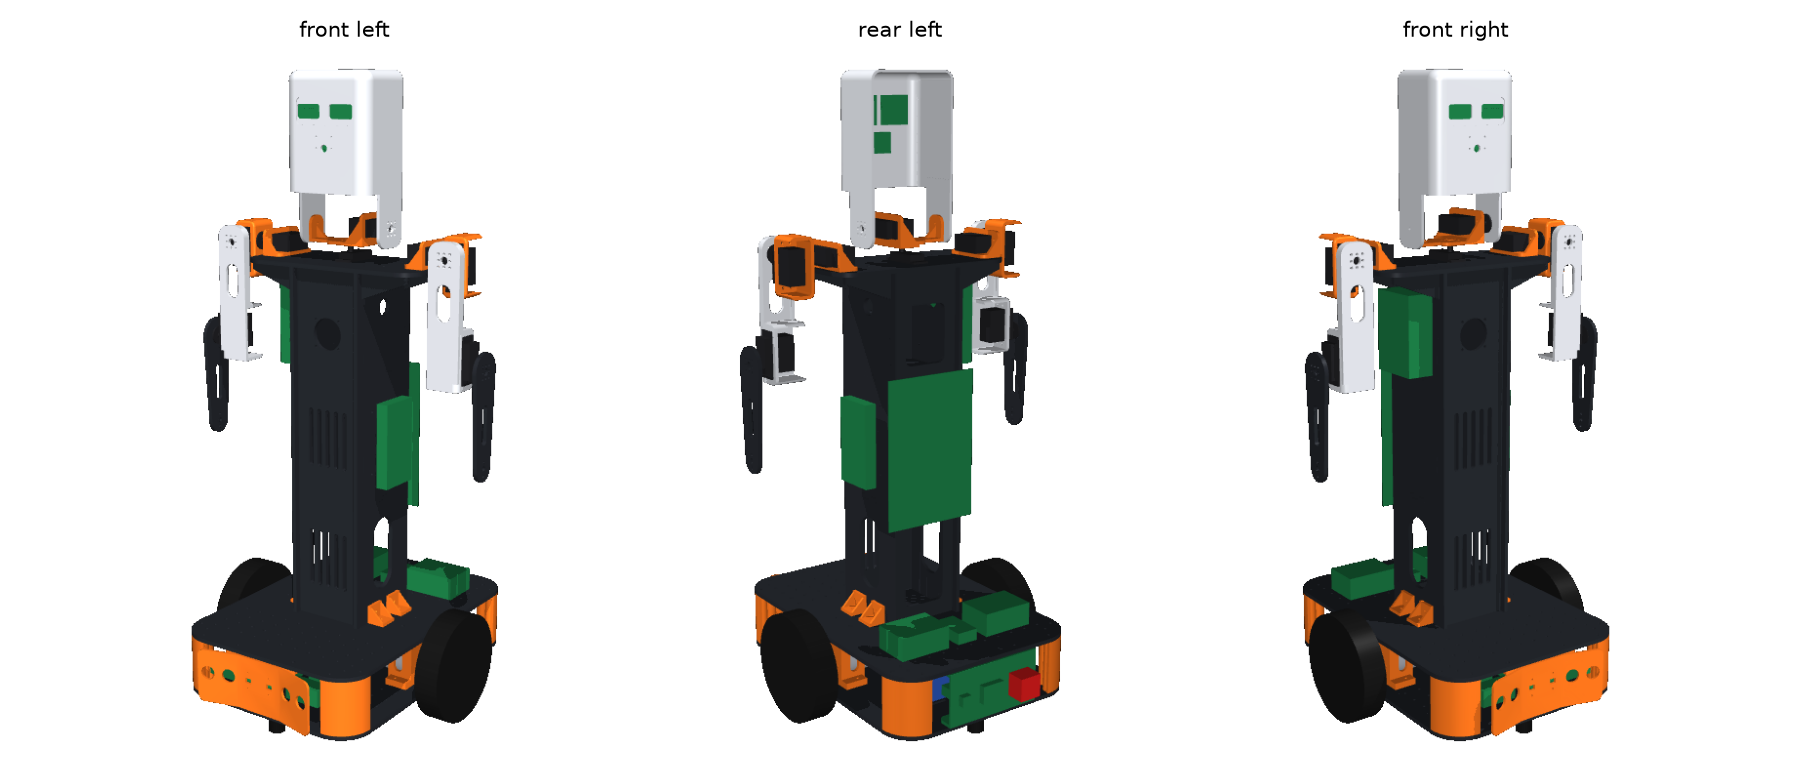
\includegraphics[width=\linewidth]{figs/v2_assembly_views.png}
\caption{Full assembly, rendered from the twin: front left, rear left, front right. Black: laser-cut plates. Orange and white: printed parts. Green: boards. Dark grey: kit actuators.}
\end{figure}

\subsection{Component placement and mounting}
Power sits low and at the rear, control sits in the torso between the base wiring and the servo wiring, and sensing sits at the front.
\begin{figure}[H]\centering
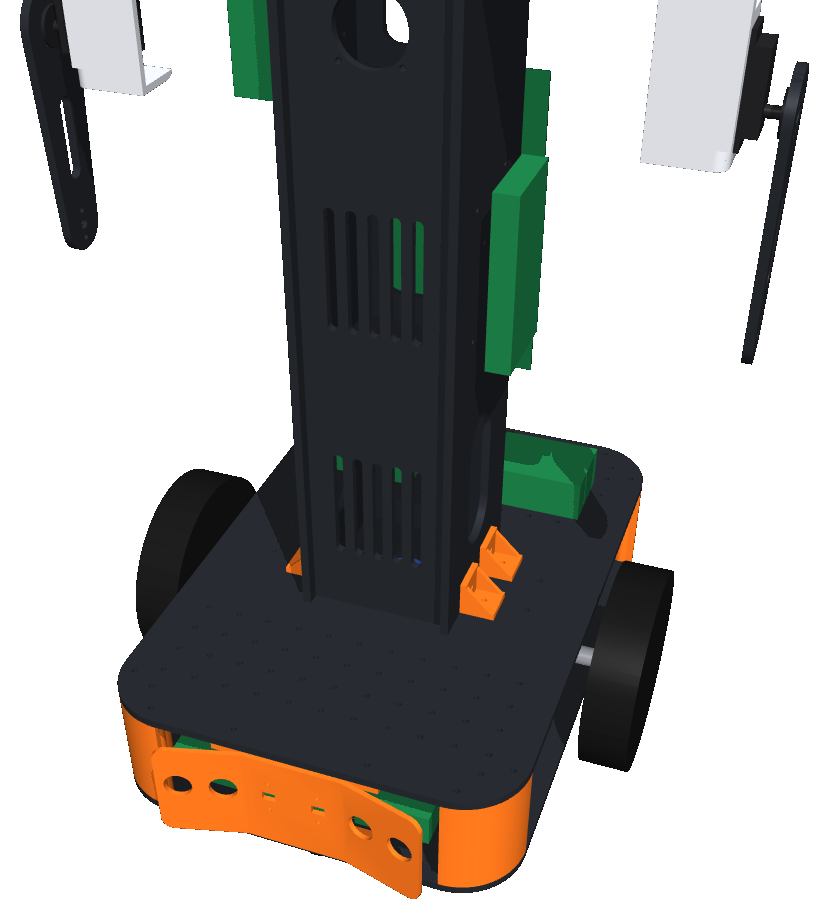
\includegraphics[width=0.62\linewidth]{figs/v2_base_view.png}
\caption{The base from the front left: drivers and sensor bar in front, battery and converters behind the axle.}
\end{figure}

\begin{table}[H]\small
\begin{tabularx}{\linewidth}{@{}P{38mm}P{56mm}L@{}}
\toprule
\textbf{Component} & \textbf{Position and mounting} & \textbf{Reason}\\
\midrule
Battery & Lower deck (L01), 95\,mm behind the axle; two straps through deck slots & Heaviest part at the lowest point; keeps the robot on its rear caster\\
Gearmotors & Printed brackets P04, M3 screws on the gearbox face and into the deck & Shaft at wheel-axle height\\
BTS7960 drivers & Lower deck front; M3 standoffs on the hole grid & Shortest high-current run; balances the battery\\
E-stop, switch & Printed control panel P07 between the decks & Reachable without crossing the arms\\
Three converters & Upper deck (L02) rear; M3 standoffs on the hole grid & Above the battery, in open air\\
MPU-6050 & Upper deck, close to the turning axis & Rigid, far from the motors\\
Arduino Mega & Left torso plate L08; M3 standoffs & Between base wiring and servo wiring\\
Raspberry Pi 5 & Right torso plate L09, top; M2.5 standoffs & Shortest path to the camera\\
PCA9685 & Torso shelf (L10) & Under the shoulders, short servo leads\\
Perfboard & Back of the torso, vertical & All eight servo plugs land in one place\\
VL53L0X, HC-SR04 & Printed front bar P06 under the upper deck & Ahead of everything\\
OLEDs, camera & Behind the head face plate (P20) & Move with the head\\
Servos & Ears screwed to a printed wall or plate, body through a window & Each servo body sits in the link before its joint\\
\bottomrule
\end{tabularx}
\end{table}

\subsection{Exploded view}
\begin{figure}[H]\centering
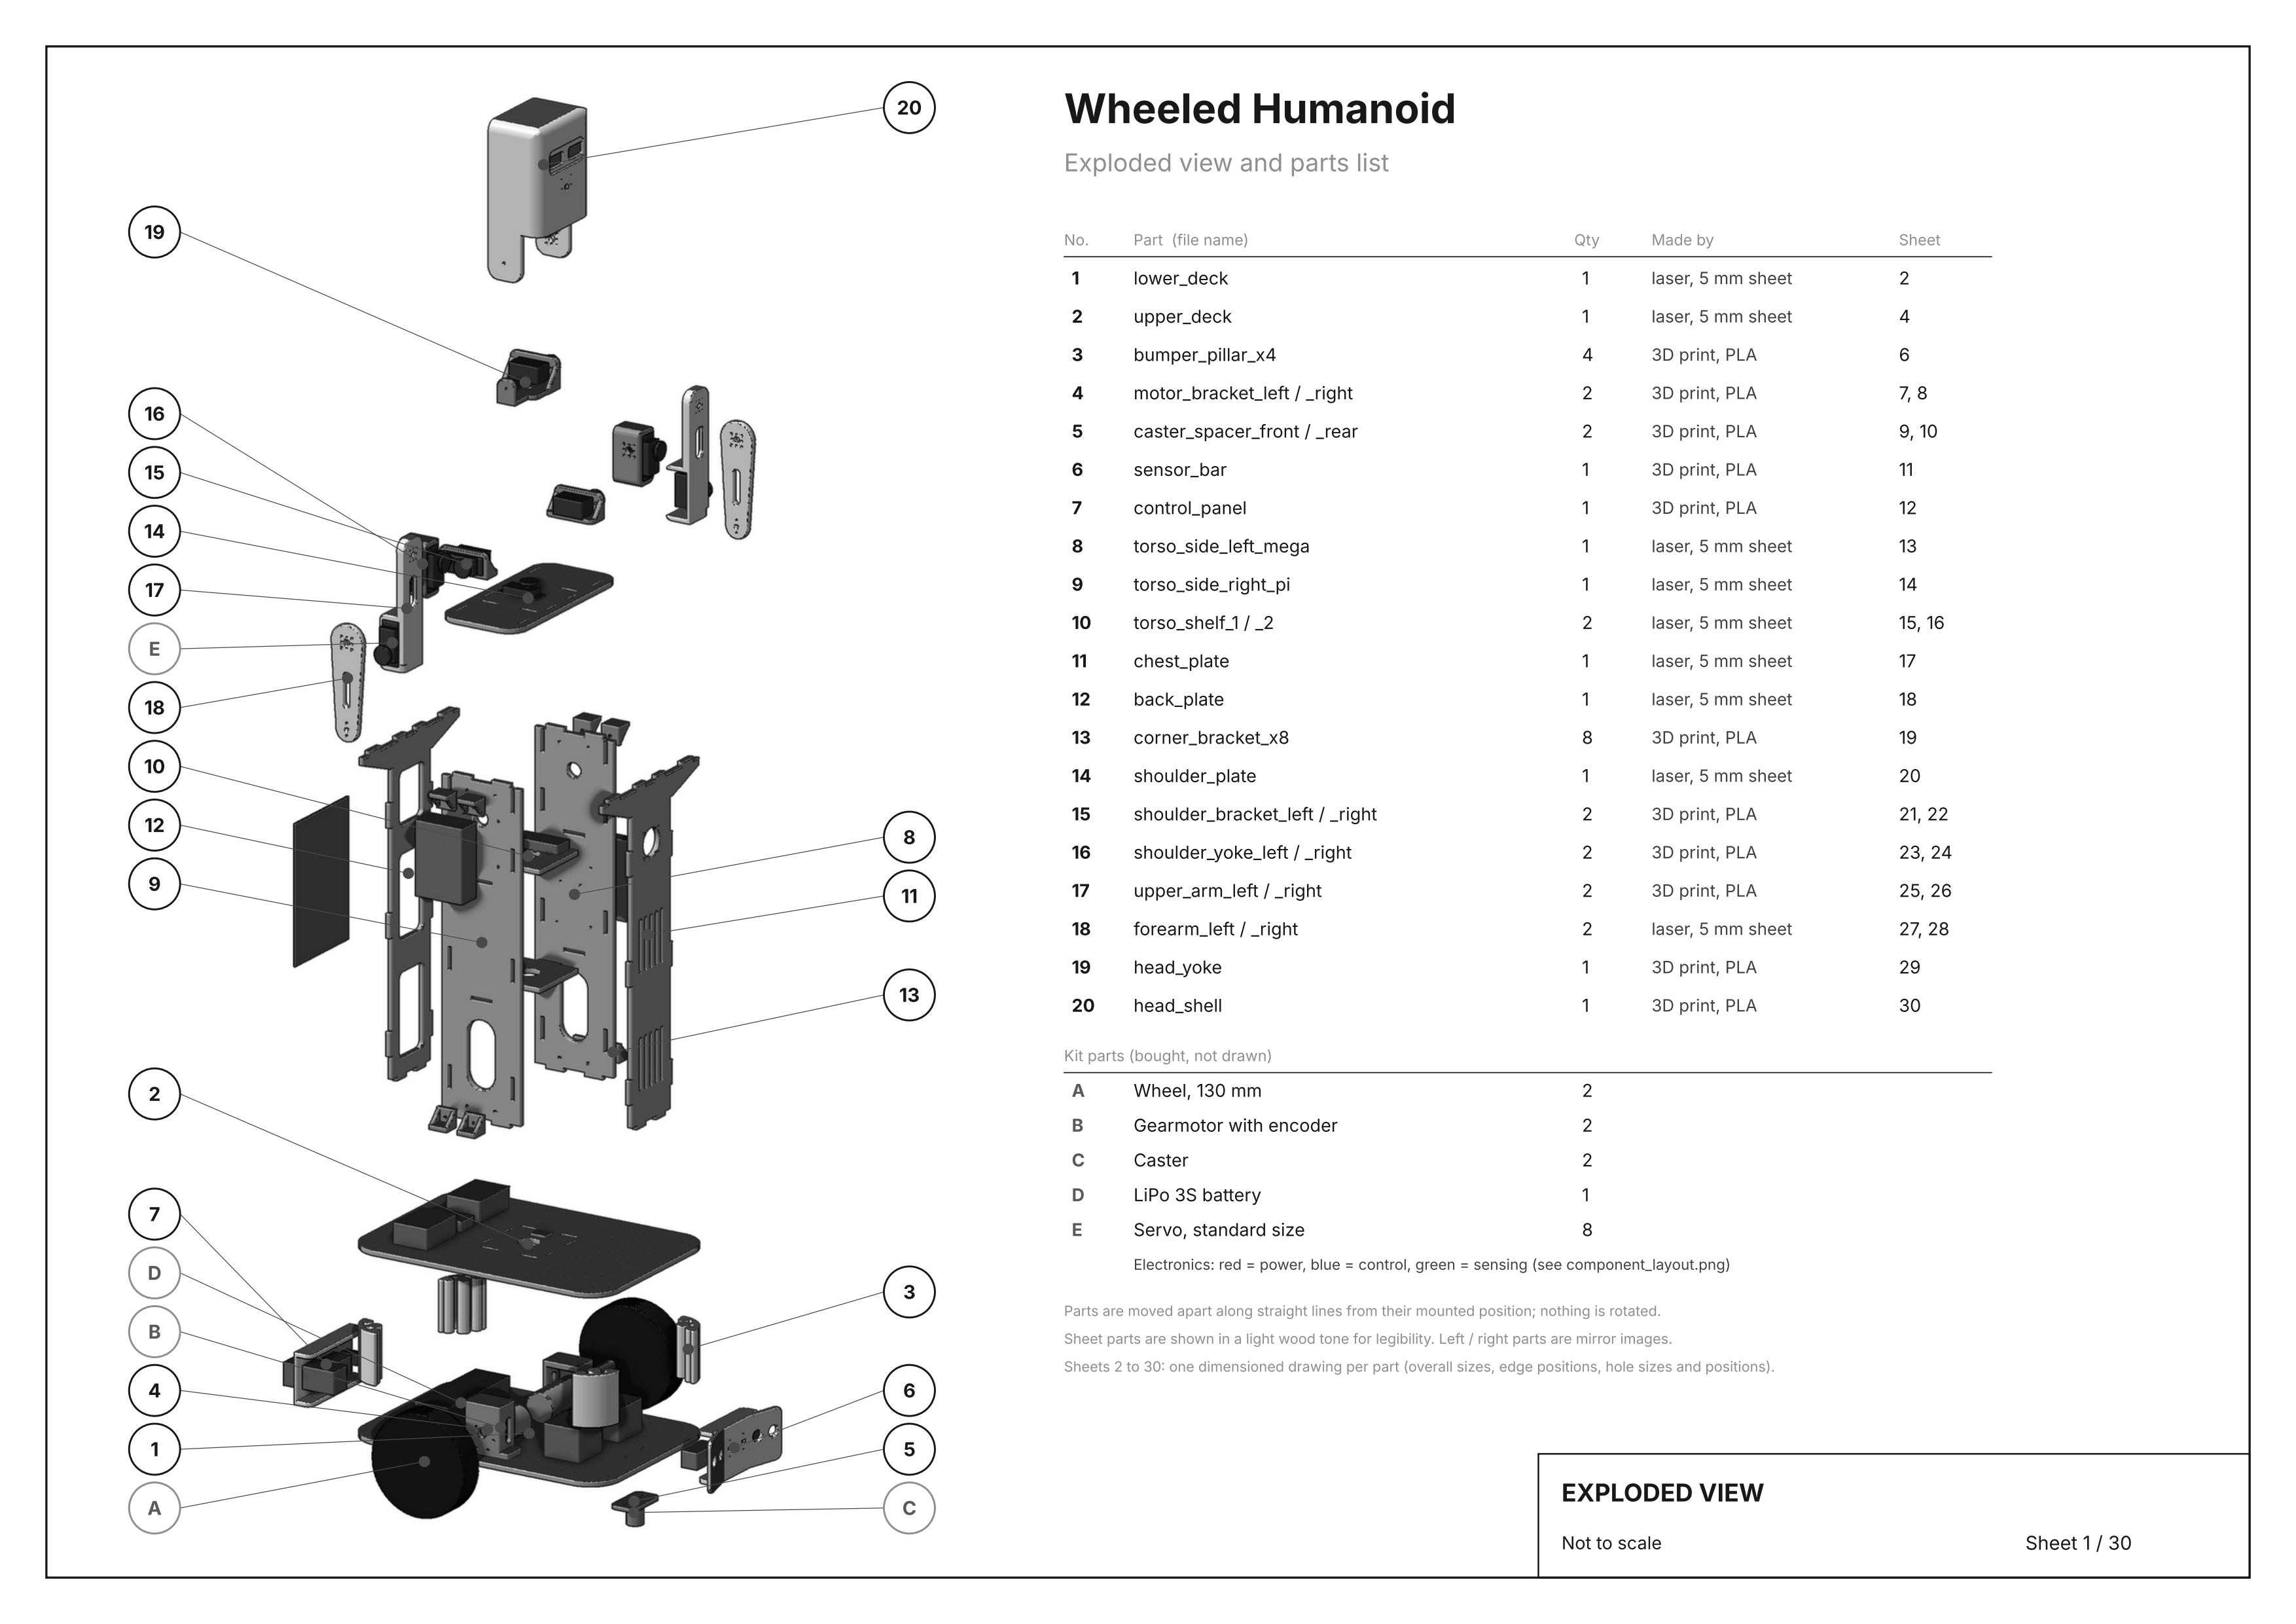
\includegraphics[width=\linewidth]{figs/drawing_sheet01.png}
\caption{Exploded view and parts list (sheet 1 of the drawings). Part numbers are those of the fabrication files.}
\end{figure}

\subsection{Dimensioned drawings of the key parts}
The complete set is 30 A4 sheets, one per part, with overall sizes, edge positions and every hole, in the \file{info/} folder of the repository. Four of them follow.
\begin{figure}[H]\centering
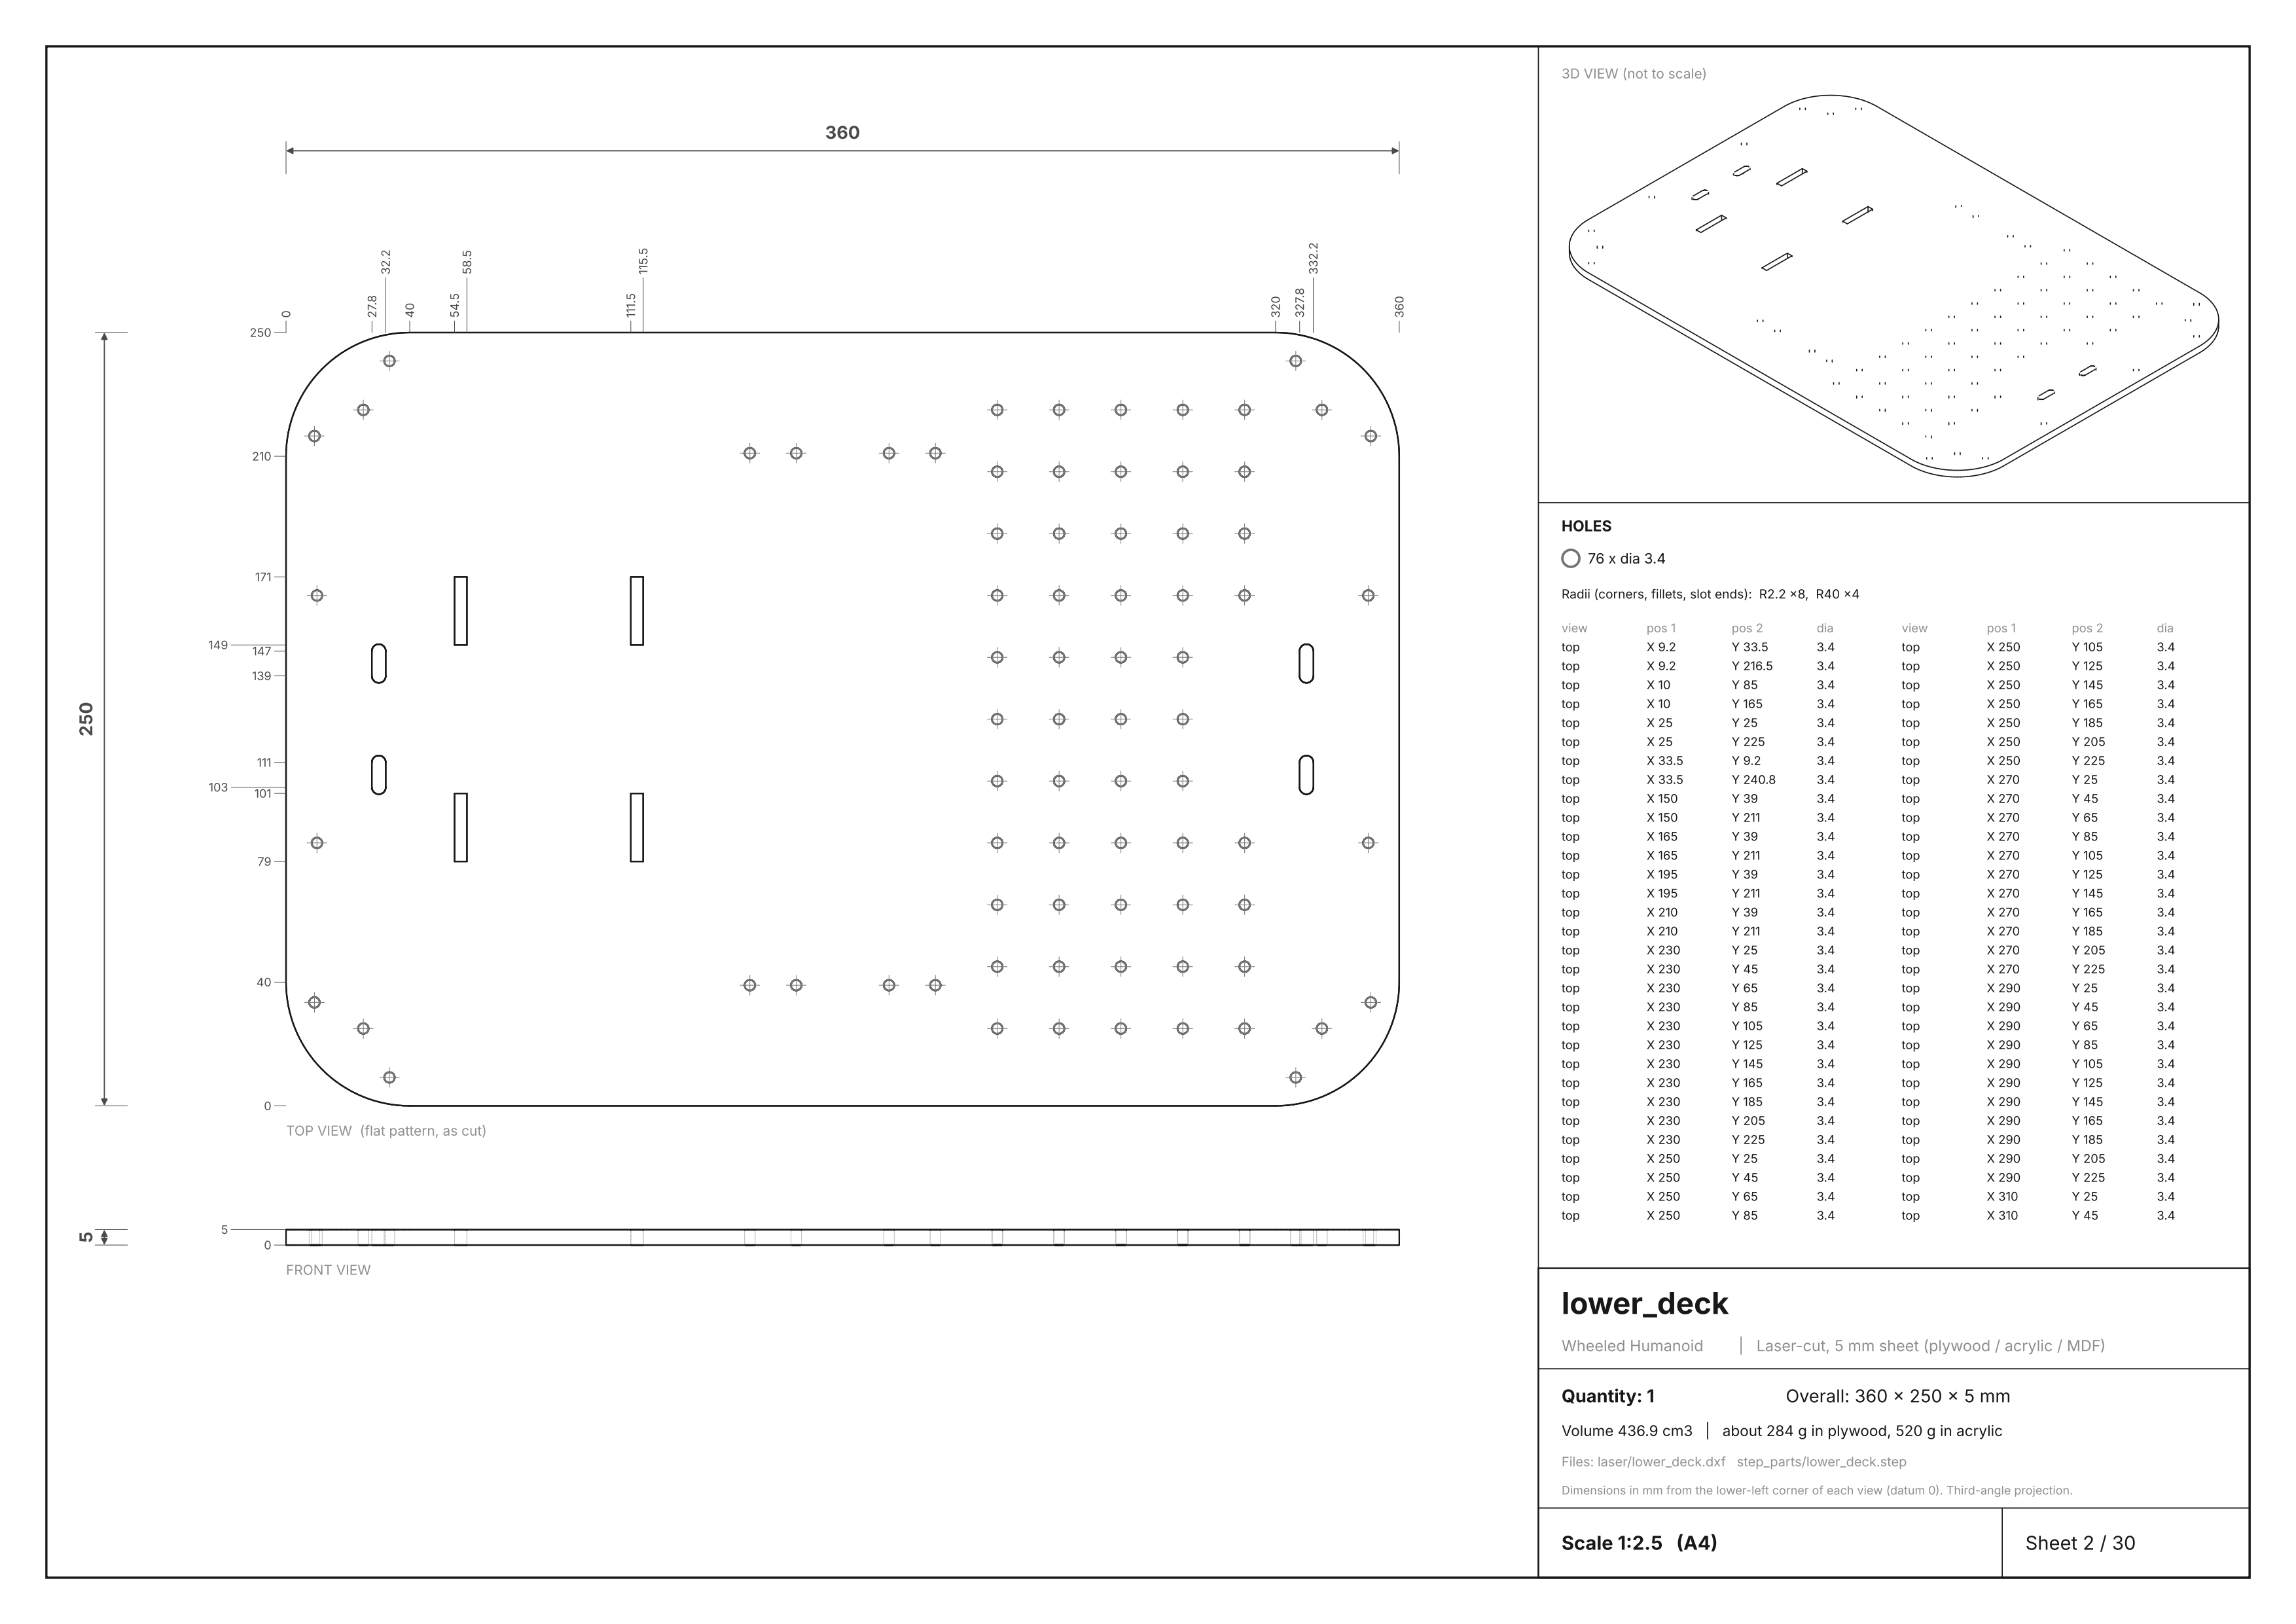
\includegraphics[width=\linewidth]{figs/drawing_sheet02.png}
\caption{L01 lower deck: motor brackets, battery straps, driver hole grid.}
\end{figure}
\begin{figure}[H]\centering
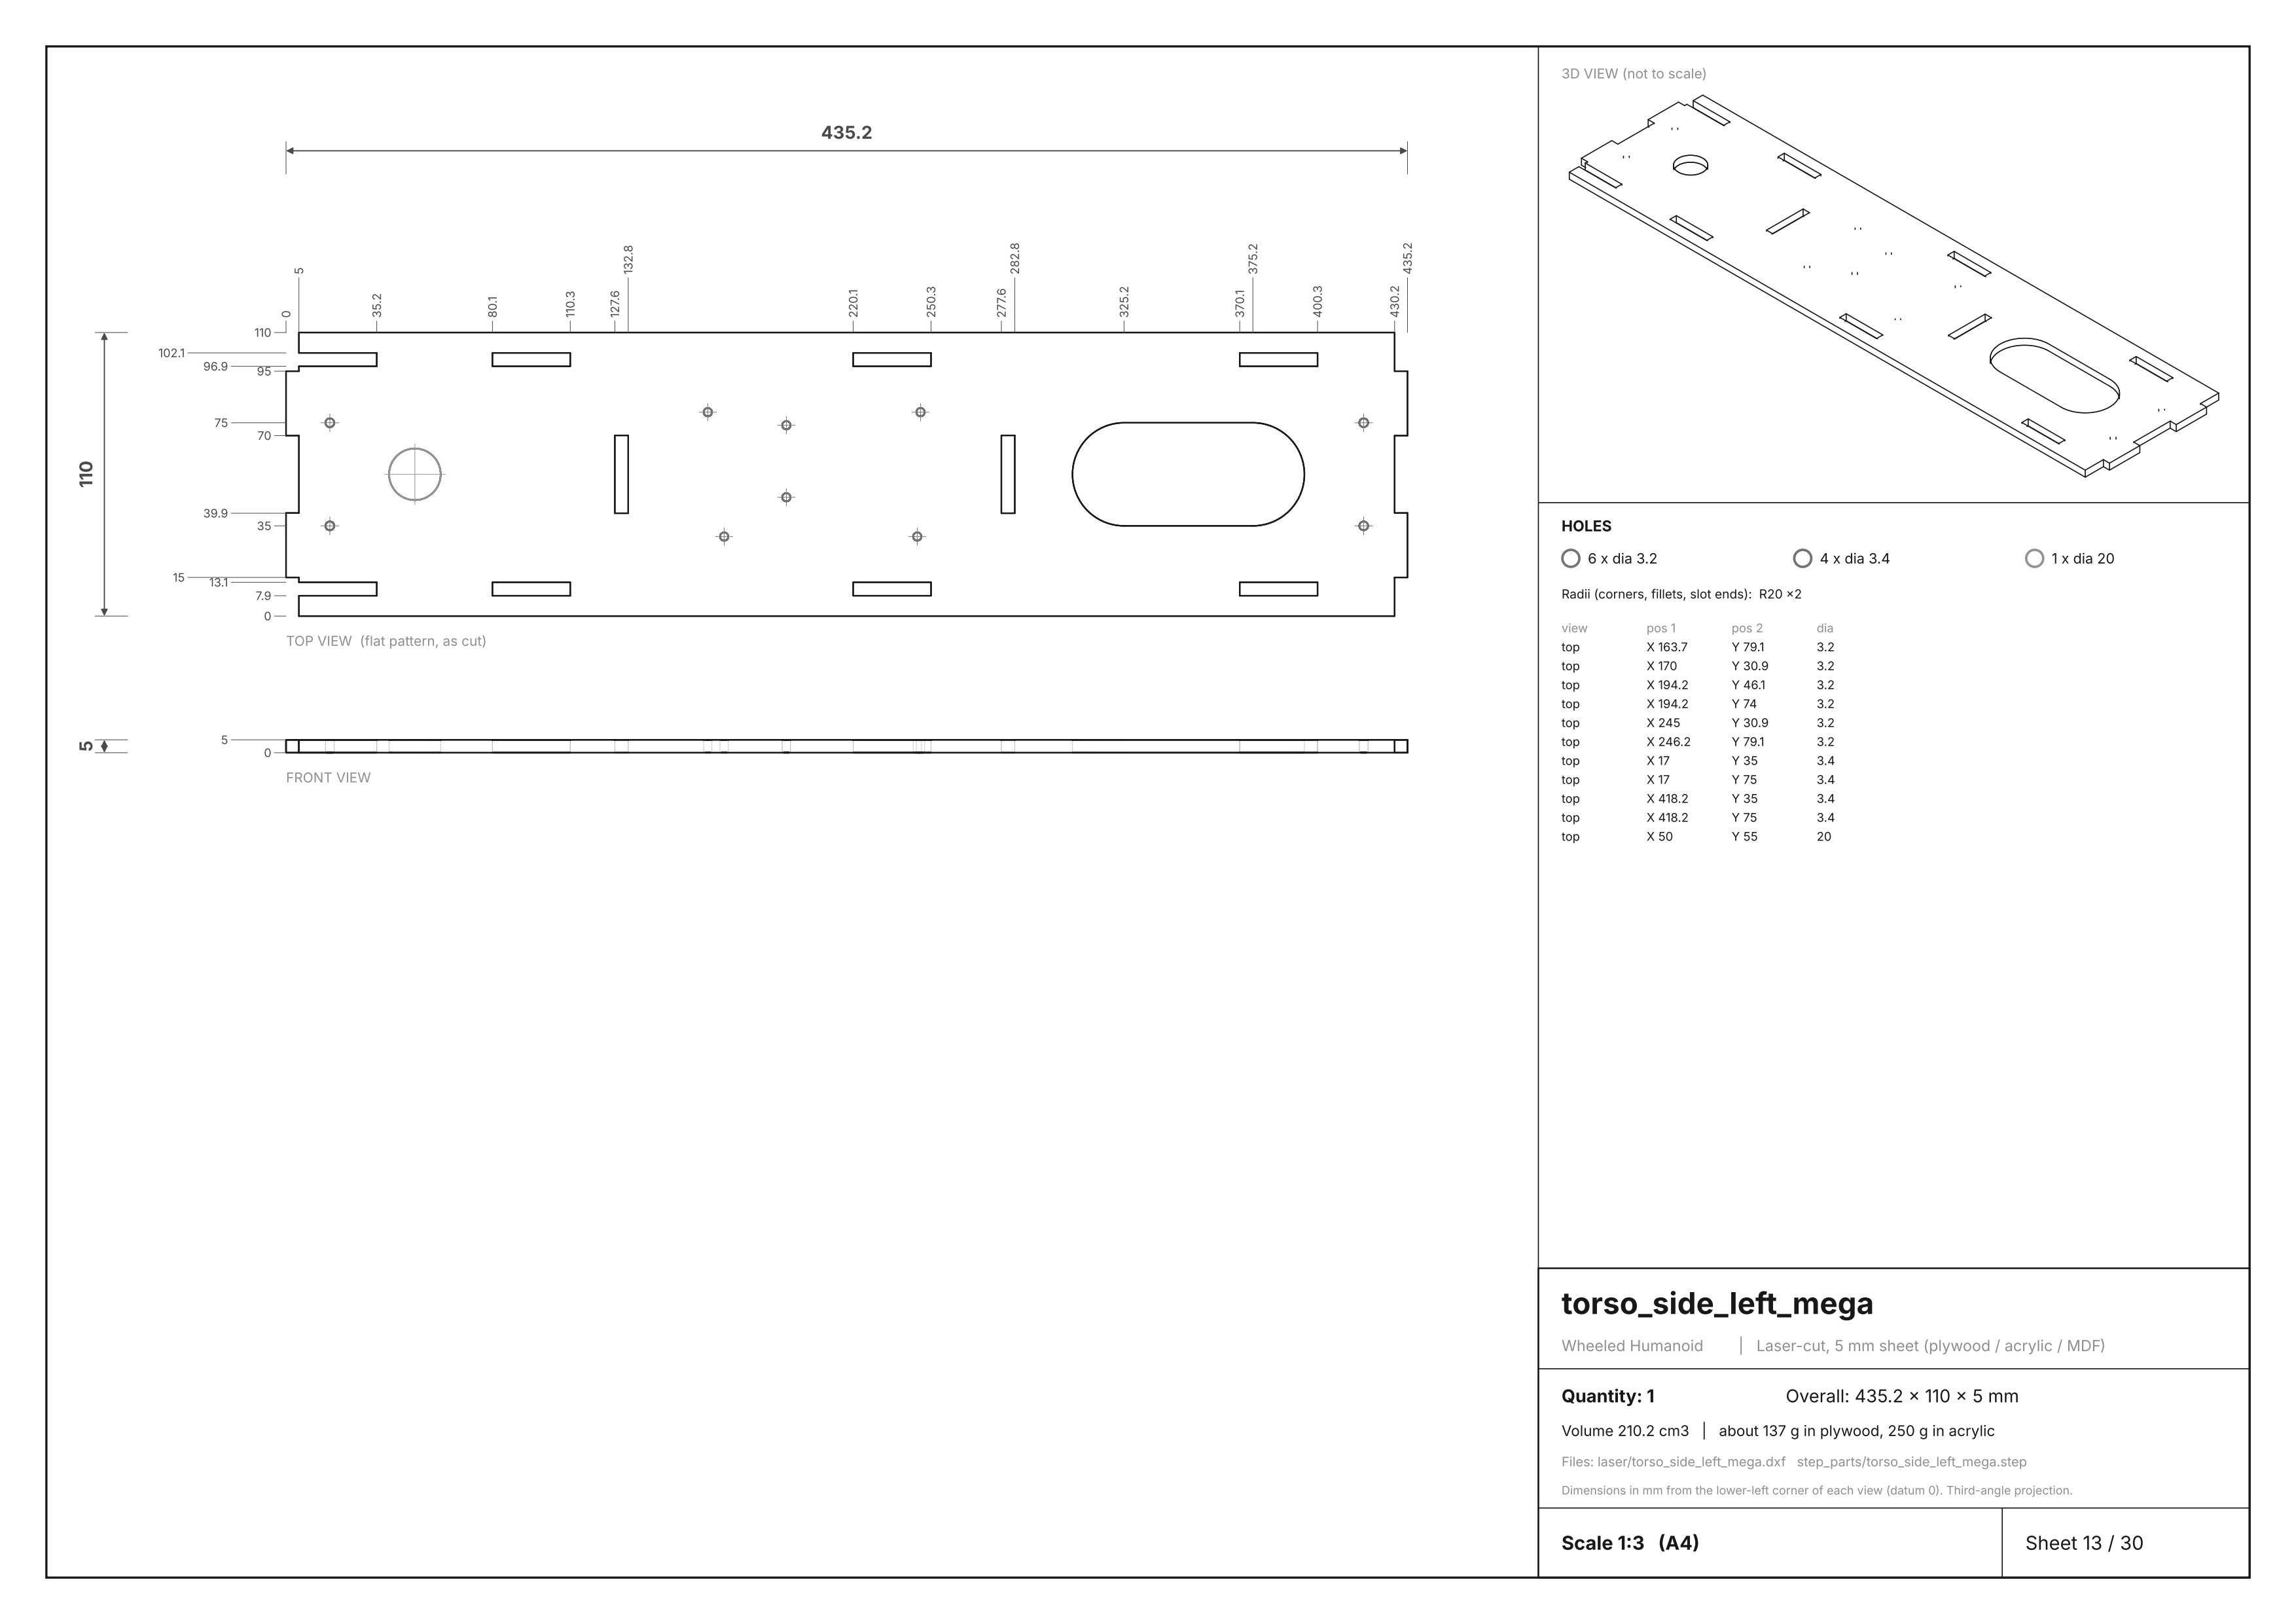
\includegraphics[width=\linewidth]{figs/drawing_sheet13.png}
\caption{L08 left torso plate (Mega side).}
\end{figure}
\begin{figure}[H]\centering
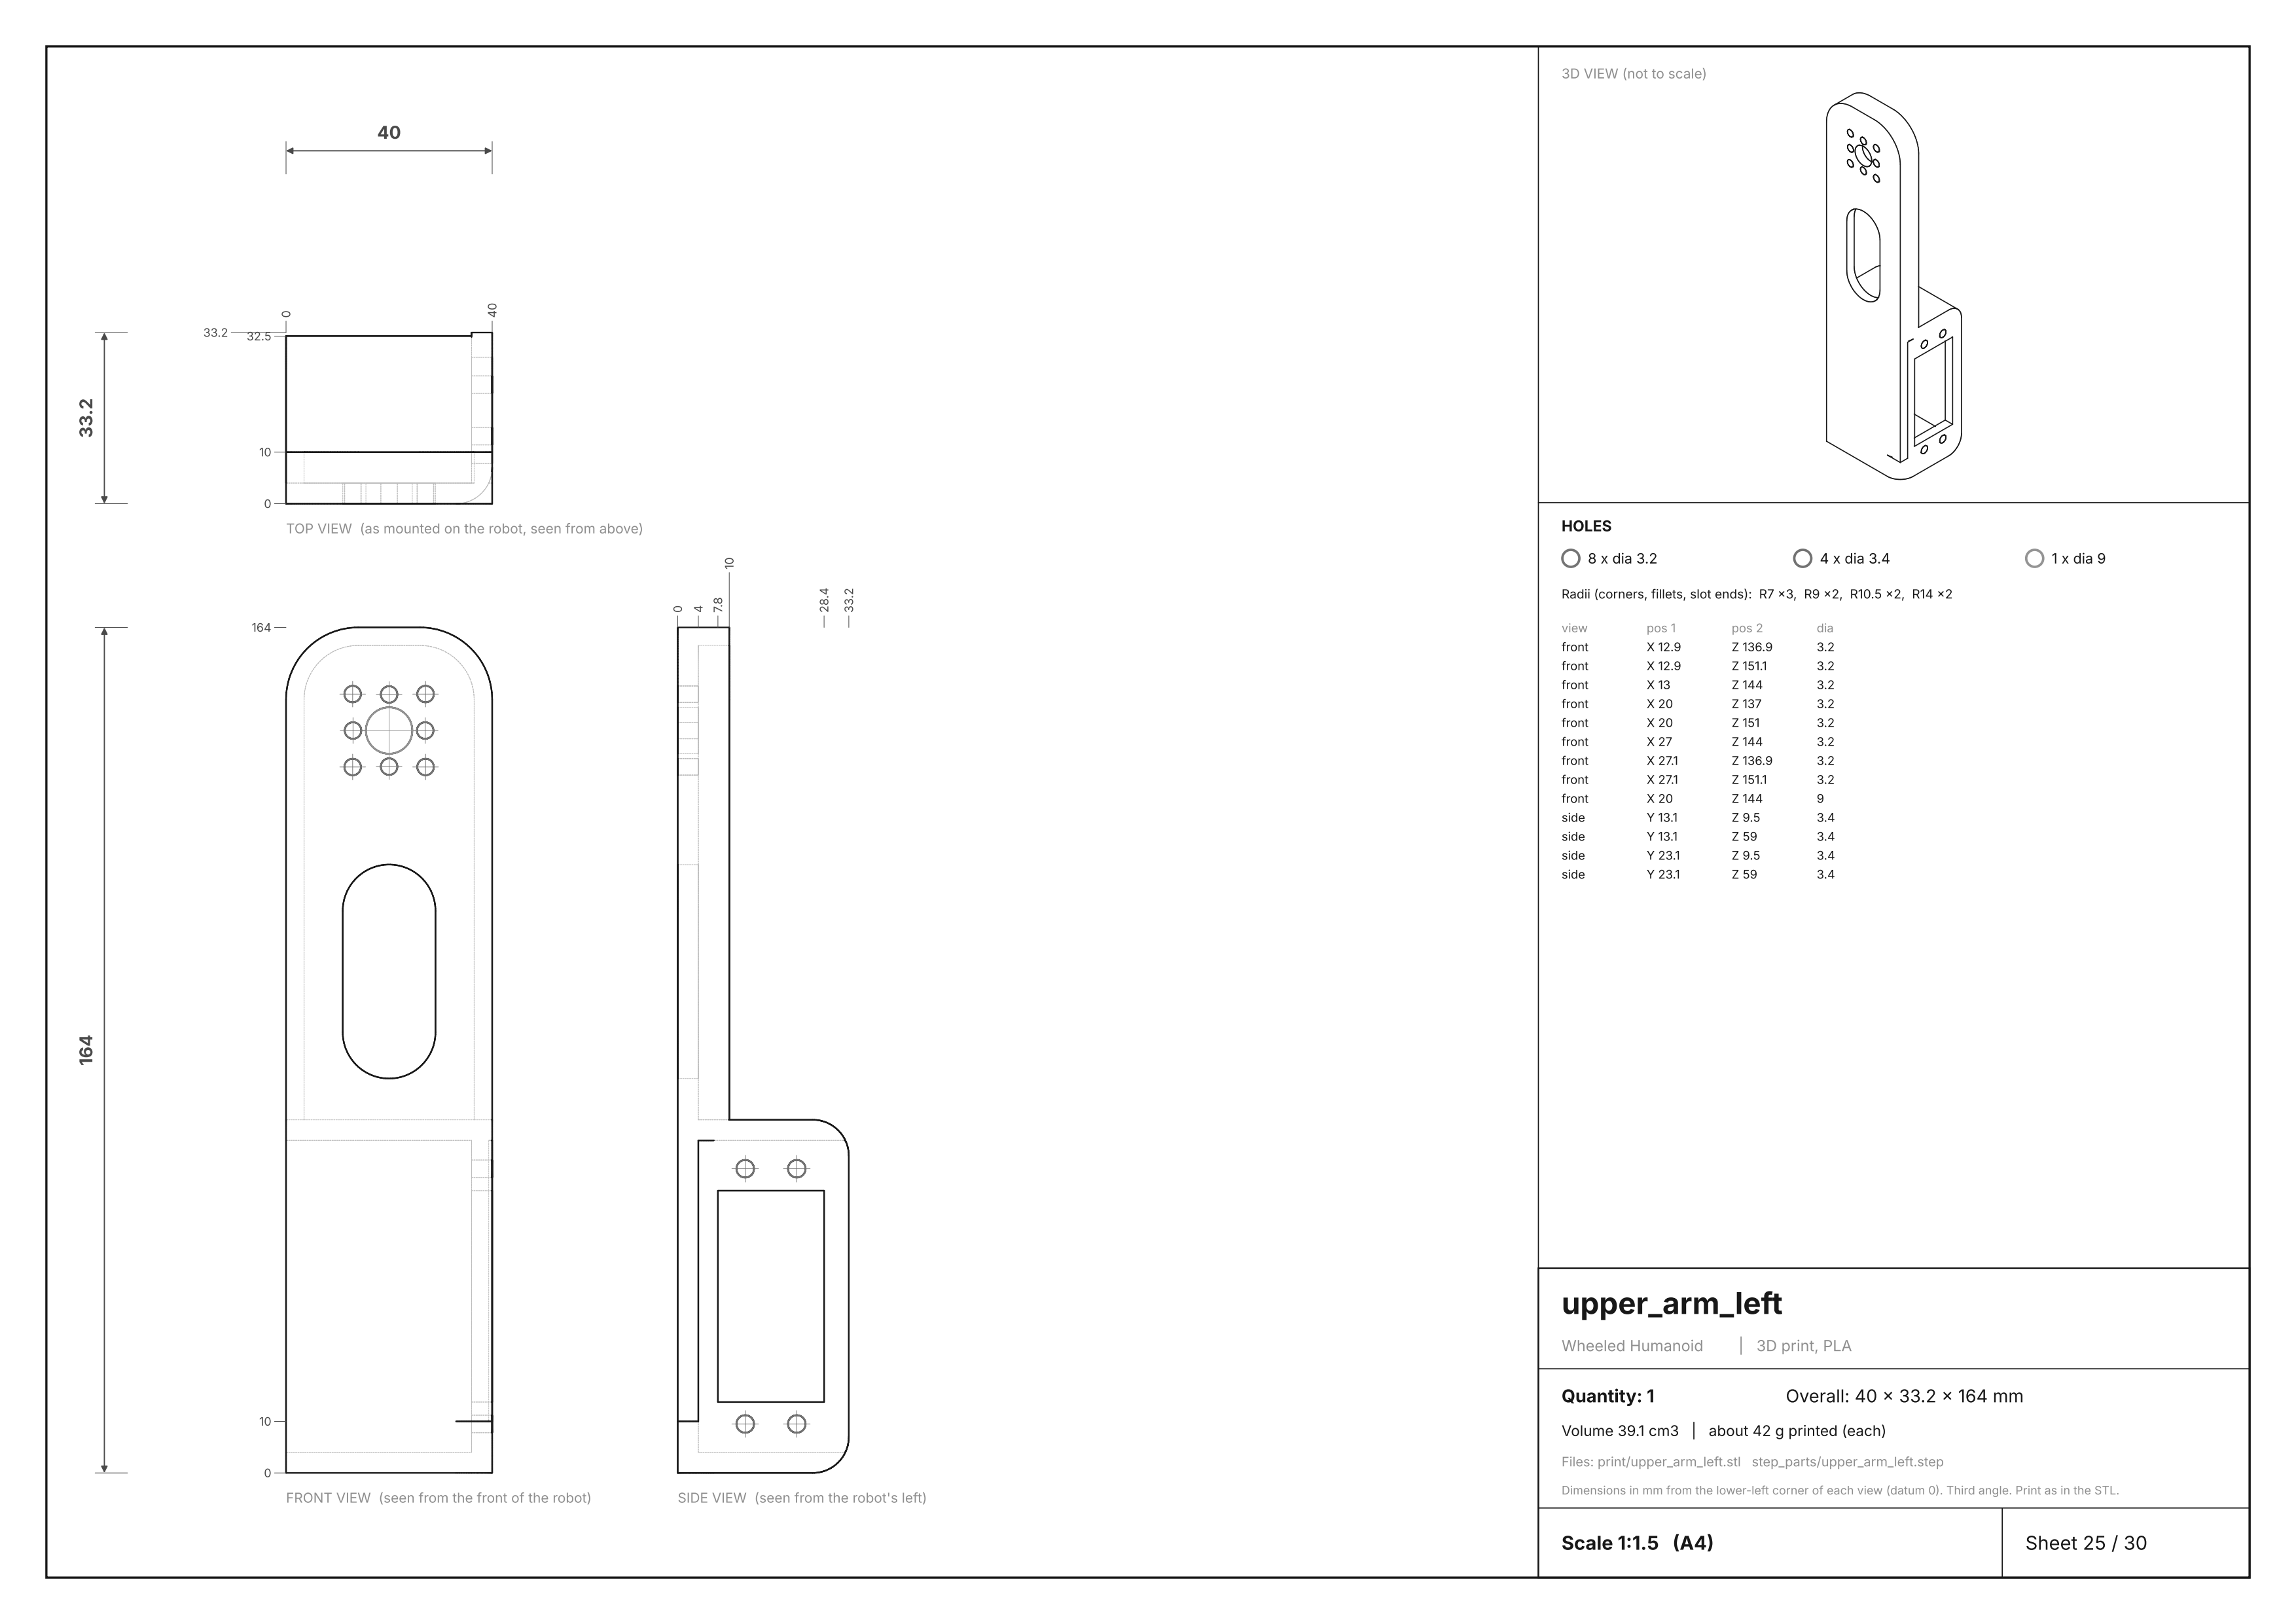
\includegraphics[width=\linewidth]{figs/drawing_sheet25.png}
\caption{P17 upper arm: roll horn at the top, elbow servo window at the bottom.}
\end{figure}
\begin{figure}[H]\centering
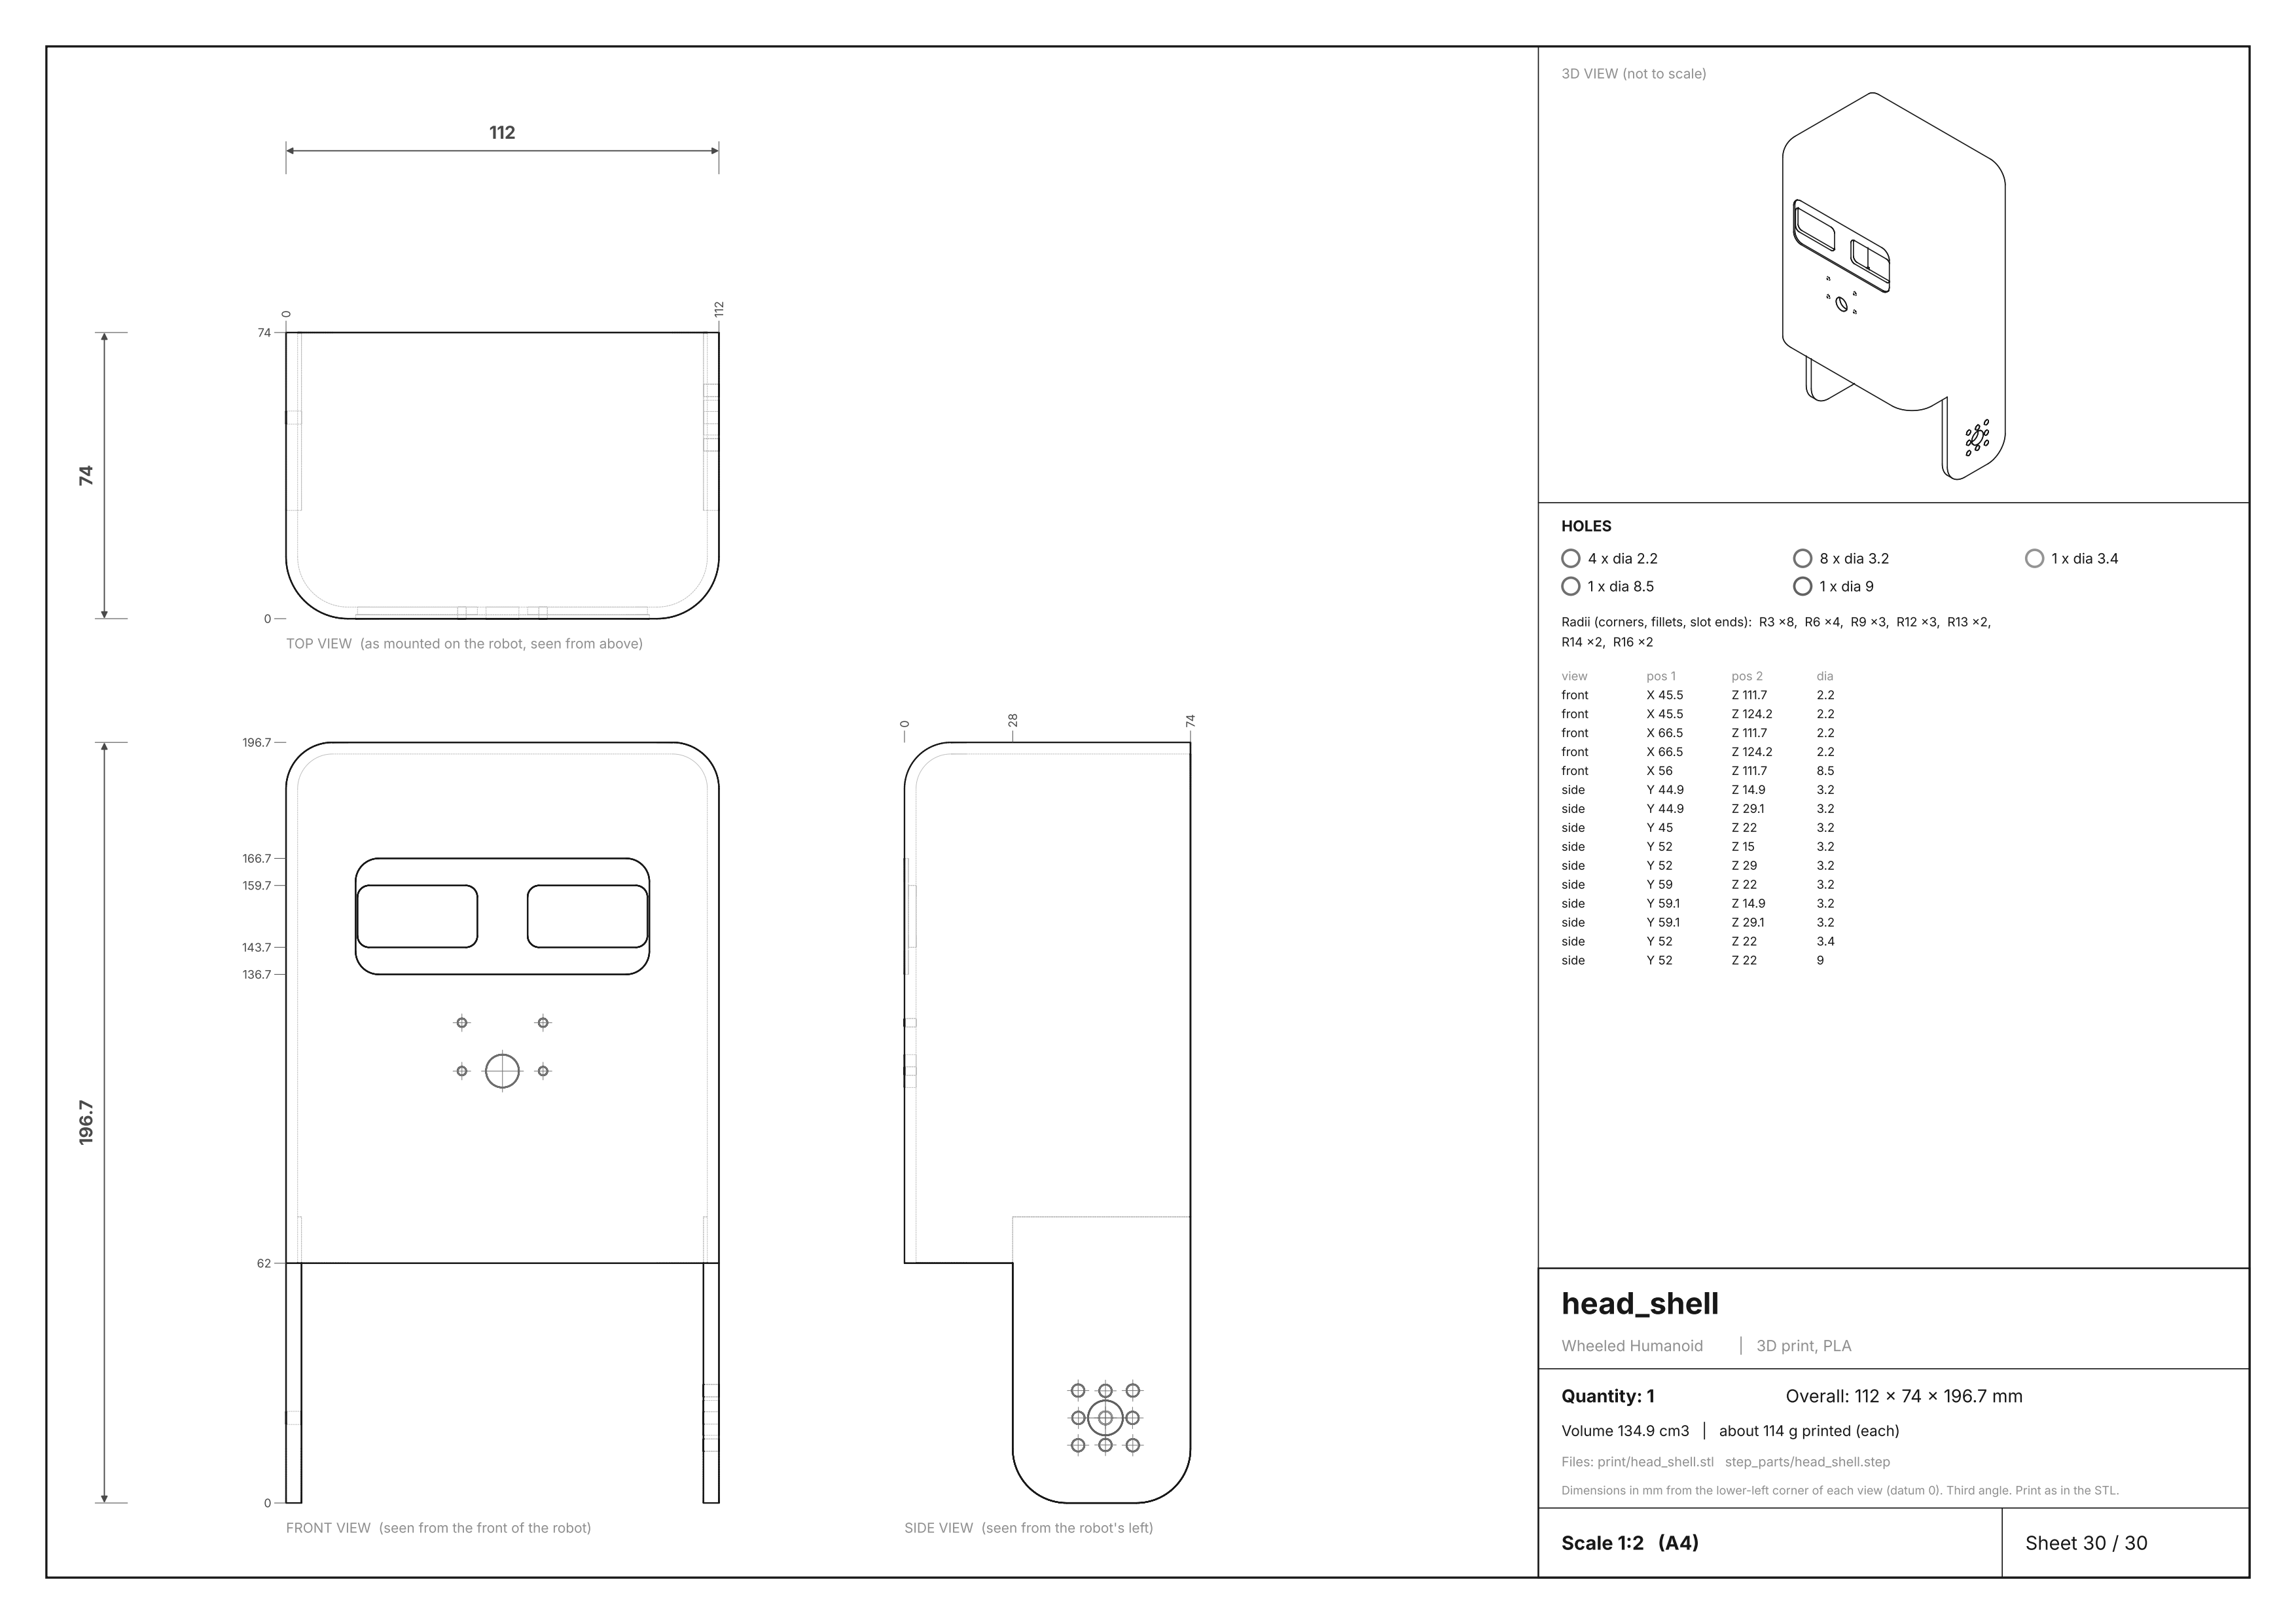
\includegraphics[width=\linewidth]{figs/drawing_sheet30.png}
\caption{P20 head shell: camera hole and OLED windows in the face, tilt horn on the side.}
\end{figure}

\subsection{Source files}
\begin{table}[H]\small
\begin{tabularx}{\linewidth}{@{}P{84mm}L@{}}
\toprule
\textbf{In the repository} & \textbf{Content}\\
\midrule
STEP, repository root & Full assembly with every kit component\\
STEP, repository root, and \file{step_parts/} & Designed parts, assembled and one STEP per part\\
\file{info/} & 30 dimensioned drawings and the exploded view\\
\file{fabrication/} & Numbered print and cut files, settings table (section~\ref{sec:fab})\\
\file{sim/}, \file{robot_viewer/} & Digital twin (URDF, MuJoCo) generated from the CAD\\
\bottomrule
\end{tabularx}
\end{table}

% =============================================================== 3 print files
\clearpage
\section{Print-ready 3D files}\label{sec:fab}
\textbf{Folder:} \url{\repo/tree/main/fabrication}. One file per part, named \file{P<no.>_<part>_x<quantity>.stl} or \file{L<no.>_<part>_x<quantity>.dxf}, where the number is the item of the drawings' parts list. Every STL is placed on the bed in its print orientation. The package and the tables below are generated by \file{fabrication/make_fabrication.py}, so they are rebuilt in one command after a CAD change.

\subsection{3D-printed parts}
16 files, 26 pieces, about 550\,g of PLA. Common settings: 0.2\,mm layers, 0.4\,mm nozzle, brim on the tall thin parts (P03, P06, P20). Everything fits a 300\,$\times$\,300\,$\times$\,300\,mm bed; the largest part is the head shell, 197\,mm tall.
% generated from fabrication/README.md (fabrication/make_fabrication.py)
{\footnotesize\setlength{\tabcolsep}{2.5pt}
\begin{longtable}{@{}lP{45mm}rrrP{25mm}P{25mm}P{21mm}r@{}}
\toprule
\textbf{No.} & \textbf{File} & \textbf{Qty} & \textbf{Infill} & \textbf{Walls} & \textbf{Orientation} & \textbf{Supports} & \textbf{Size on bed (mm)} & \textbf{g}\\
\midrule\endhead
P03 & {\scriptsize\nolinkurl{P03_bumper_pillar_x4.stl}} & 4 & 40\,\% & 4 & as designed: 6 cm\textsuperscript{2} flat on the bed & none & 40\,$\times$\,40\,$\times$\,65 & 30\\
P04 & {\scriptsize\nolinkurl{P04_motor_bracket_left_x1.stl}} & 1 & 50\,\% & 4 & as designed: 31 cm\textsuperscript{2} flat on the bed & none & 72\,$\times$\,65\,$\times$\,33 & 38\\
P04 & {\scriptsize\nolinkurl{P04_motor_bracket_right_x1.stl}} & 1 & 50\,\% & 4 & as designed: 31 cm\textsuperscript{2} flat on the bed & none & 72\,$\times$\,65\,$\times$\,33 & 38\\
P05 & {\scriptsize\nolinkurl{P05_caster_spacer_front_x1.stl}} & 1 & 100\,\% & 3 & as designed: 18 cm\textsuperscript{2} flat on the bed & none & 32\,$\times$\,60\,$\times$\,3 & 8\\
P05 & {\scriptsize\nolinkurl{P05_caster_spacer_rear_x1.stl}} & 1 & 100\,\% & 3 & as designed: 18 cm\textsuperscript{2} flat on the bed & none & 32\,$\times$\,60\,$\times$\,3 & 8\\
P06 & {\scriptsize\nolinkurl{P06_sensor_bar_x1.stl}} & 1 & 25\,\% & 3 & as designed: 24 cm\textsuperscript{2} flat on the bed & none (bridges up to 20 mm) & 36\,$\times$\,160\,$\times$\,65 & 33\\
P07 & {\scriptsize\nolinkurl{P07_control_panel_x1.stl}} & 1 & 40\,\% & 4 & as designed: 69 cm\textsuperscript{2} flat on the bed & none & 65\,$\times$\,124\,$\times$\,22 & 35\\
P13 & {\scriptsize\nolinkurl{P13_corner_bracket_x8.stl}} & 8 & 60\,\% & 4 & as designed: 5 cm\textsuperscript{2} flat on the bed & none & 24\,$\times$\,22\,$\times$\,22 & 5\\
P15 & {\scriptsize\nolinkurl{P15_shoulder_bracket_left_x1.stl}} & 1 & 40\,\% & 4 & turned: flat contact 11.3 to 17 cm\textsuperscript{2} & none & 66\,$\times$\,26\,$\times$\,31 & 10\\
P15 & {\scriptsize\nolinkurl{P15_shoulder_bracket_right_x1.stl}} & 1 & 40\,\% & 4 & turned: flat contact 11.3 to 17 cm\textsuperscript{2} & none & 66\,$\times$\,26\,$\times$\,31 & 10\\
P16 & {\scriptsize\nolinkurl{P16_shoulder_yoke_left_x1.stl}} & 1 & 40\,\% & 4 & turned: flat contact 0.6 to 17 cm\textsuperscript{2}, bridging 20 to 3 cm\textsuperscript{2} & none (bridges up to 35 mm) & 36\,$\times$\,68\,$\times$\,31 & 17\\
P16 & {\scriptsize\nolinkurl{P16_shoulder_yoke_right_x1.stl}} & 1 & 40\,\% & 4 & turned: flat contact 0.6 to 17 cm\textsuperscript{2}, bridging 20 to 3 cm\textsuperscript{2} & none (bridges up to 35 mm) & 36\,$\times$\,68\,$\times$\,31 & 17\\
P17 & {\scriptsize\nolinkurl{P17_upper_arm_left_x1.stl}} & 1 & 30\,\% & 4 & as designed: 56 cm\textsuperscript{2} flat on the bed & none & 164\,$\times$\,40\,$\times$\,33 & 33\\
P17 & {\scriptsize\nolinkurl{P17_upper_arm_right_x1.stl}} & 1 & 30\,\% & 4 & as designed: 56 cm\textsuperscript{2} flat on the bed & none & 164\,$\times$\,40\,$\times$\,33 & 33\\
P19 & {\scriptsize\nolinkurl{P19_head_yoke_x1.stl}} & 1 & 40\,\% & 4 & as designed: 35 cm\textsuperscript{2} flat on the bed & none & 66\,$\times$\,84\,$\times$\,37 & 22\\
P20 & {\scriptsize\nolinkurl{P20_head_shell_x1.stl}} & 1 & 15\,\% & 3 & as designed: 56 cm\textsuperscript{2} flat on the bed & build plate only, under the rounded lower edge (first 4 mm) & 74\,$\times$\,112\,$\times$\,197 & 90\\
\bottomrule
\end{longtable}}

\textbf{How the settings were chosen.} Infill and walls follow the load: 50\,\% and four walls on the motor brackets, which carry the robot's weight and the motor torque; 40\,\% and four walls on every part that holds a servo; 60\,\% on the small corner brackets that join the torso; 100\,\% on the 3.5\,mm caster shims; 15\,\% on the cosmetic head shell. Masses assume PLA at 1.24\,g/cm\textsuperscript{3} with the walls solid.

\textbf{How the orientation was chosen.} The script tries the six flat orientations and the stable poses of each part and keeps the one with the least unsupported overhang (faces steeper than 45\deg), then the largest flat contact with the bed, then the lowest height; on a tie it keeps the designed orientation. Holes and slots up to 10\,mm wide print without support and flat spans up to 45\,mm are bridged. 13 parts keep their designed orientation; the shoulder brackets (P15) and shoulder yokes (P16) were turned, the yokes from 0.6 to 17\,cm\textsuperscript{2} of contact. Only the head shell needs support, on the build plate under its rounded lower edge.
\begin{figure}[H]\centering
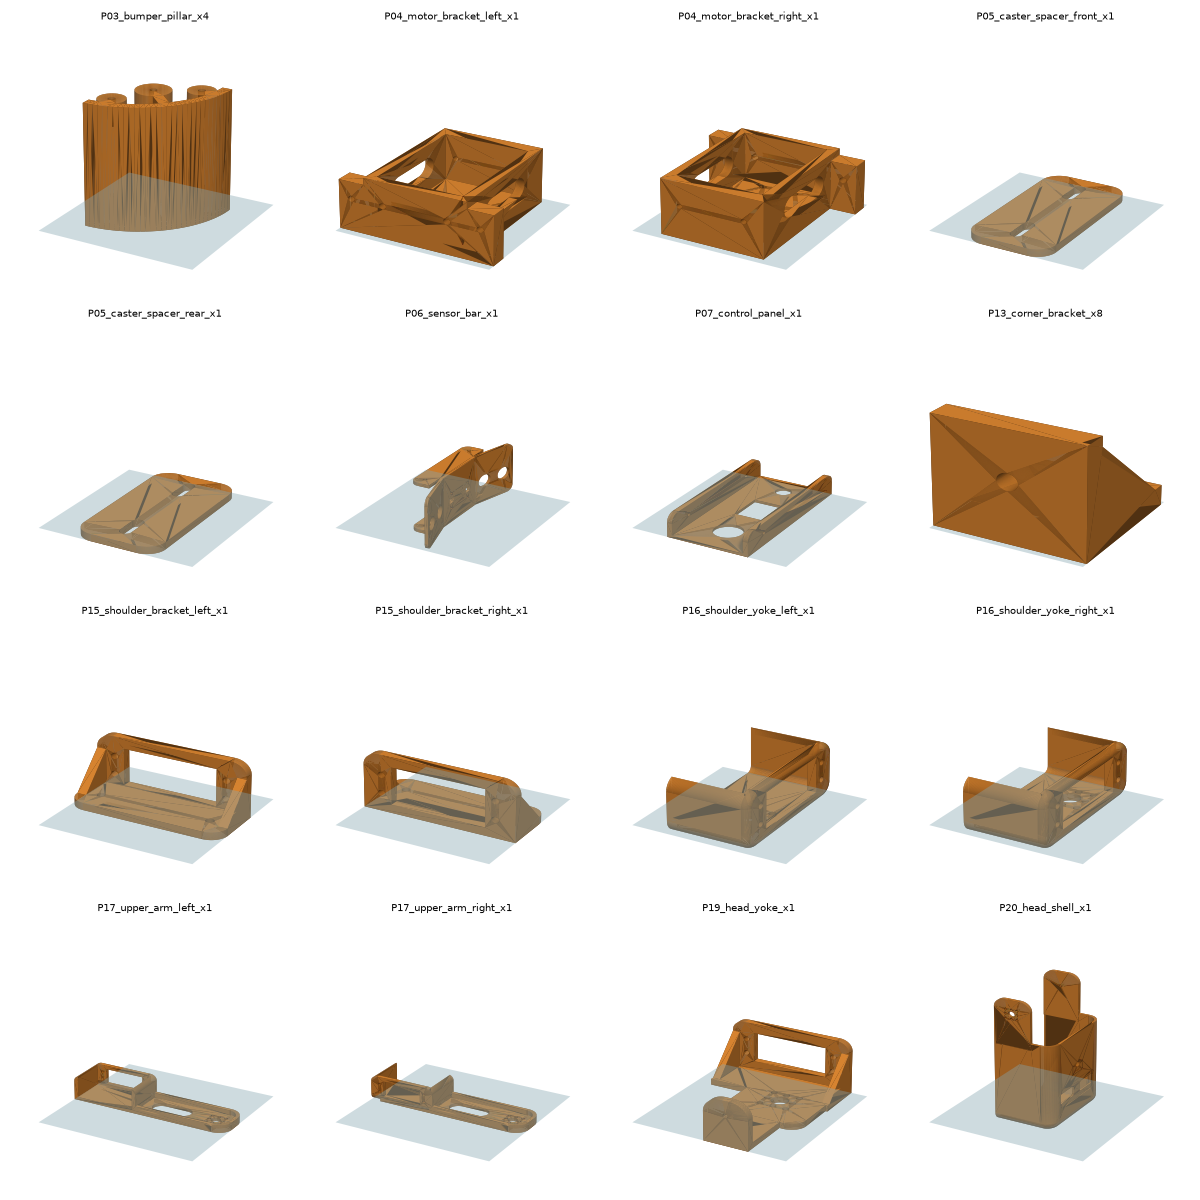
\includegraphics[width=0.86\linewidth]{figs/v2_print_orientations.png}
\caption{Every printed part as it sits on the bed (light blue).}
\end{figure}

\subsection{Laser-cut parts}
11 plates, one piece each, 5\,mm sheet, about 18.4\,m of cut. DXF in mm at 1:1, outline and holes only; the laser bed must take a 435\,mm part (L08, L09, L11, L12).
% generated from fabrication/README.md (fabrication/make_fabrication.py)
\begin{table}[H]\small
\begin{tabularx}{\linewidth}{@{}lLrlrrr@{}}
\toprule
\textbf{No.} & \textbf{File} & \textbf{Qty} & \textbf{Size (mm)} & \textbf{Holes} & \textbf{Cut (m)} & \textbf{vs CAD}\\
\midrule
L01 & {\scriptsize\nolinkurl{L01_lower_deck_x1.dxf}} & 1 & 360.0\,$\times$\,250.0 & 84 & 2.29 & +0.01\,\%\\
L02 & {\scriptsize\nolinkurl{L02_upper_deck_x1.dxf}} & 1 & 360.0\,$\times$\,250.0 & 121 & 2.89 & +0.01\,\%\\
L08 & {\scriptsize\nolinkurl{L08_torso_side_left_mega_x1.dxf}} & 1 & 110.0\,$\times$\,435.2 & 20 & 2.19 & +0.00\,\%\\
L09 & {\scriptsize\nolinkurl{L09_torso_side_right_pi_x1.dxf}} & 1 & 110.0\,$\times$\,435.2 & 18 & 2.16 & +0.00\,\%\\
L10 & {\scriptsize\nolinkurl{L10_torso_shelf_1_x1.dxf}} & 1 & 83.4\,$\times$\,95.0 & 1 & 0.45 & +0.01\,\%\\
L10 & {\scriptsize\nolinkurl{L10_torso_shelf_2_x1.dxf}} & 1 & 83.4\,$\times$\,95.0 & 1 & 0.45 & +0.01\,\%\\
L11 & {\scriptsize\nolinkurl{L11_chest_plate_x1.dxf}} & 1 & 435.2\,$\times$\,216.0 & 15 & 3.0 & +0.00\,\%\\
L12 & {\scriptsize\nolinkurl{L12_back_plate_x1.dxf}} & 1 & 435.2\,$\times$\,216.0 & 3 & 2.23 & +0.00\,\%\\
L14 & {\scriptsize\nolinkurl{L14_shoulder_plate_x1.dxf}} & 1 & 110.0\,$\times$\,236.0 & 25 & 1.59 & +0.01\,\%\\
L18 & {\scriptsize\nolinkurl{L18_forearm_left_x1.dxf}} & 1 & 44.0\,$\times$\,147.0 & 13 & 0.59 & +0.02\,\%\\
L18 & {\scriptsize\nolinkurl{L18_forearm_right_x1.dxf}} & 1 & 44.0\,$\times$\,147.0 & 13 & 0.59 & +0.02\,\%\\
\bottomrule
\end{tabularx}
\end{table}

\textbf{Every DXF is checked against the CAD.} The script cuts each plate's solid at mid-thickness and compares the net area and the number of holes with the DXF. This check found that the two forearm files held an edge view of the part (38\,$\times$\,5\,mm) instead of the 147\,$\times$\,44\,mm plate; they were regenerated from the solid, with round holes written as true circles, and now match drawing sheets 27 and 28.

% =============================================================== 4 simulation
\clearpage
\section{Simulation}\label{sec:sim}
Four levels of simulation support the design decisions, from the fastest to the most complete: unit tests of the controller against a motor model, static torque and stability from the twin, the real firmware driving a physics twin of the whole robot, and a clearance check on the exact CAD solids. All of it runs from the repository with one command each.

\subsection{Controller tests against a motor model}
The controller (\file{firmware/lib/robot_core}) contains no Arduino code, so it compiles on a computer and runs against a first-order motor model in 30 automated tests (\file{make -C firmware test}).
\begin{table}[H]\small
\begin{tabularx}{\linewidth}{@{}P{56mm}LP{38mm}@{}}
\toprule
\textbf{Test} & \textbf{Result} & \textbf{Criterion}\\
\midrule
\texttt{FWD 200}, then \texttt{BACK 50} & 1.999\,m, then 1.500\,m & error under 2\,cm\\
\texttt{TURN 90} & 89.7\deg, centre moved 0.2\,mm & error under 2\deg\\
Motor time constant 0.1 to 0.35\,s & worst error 0.8\,mm and 0.3\deg & under 1\,cm and 1\deg\\
Speed and acceleration & peak 0.41\,m/s; 0.8\,m/s\textsuperscript{2} for 0.1\,s at start & cap 0.40, profile 0.5\\
Obstacle stop from 0.40\,m/s & stops 381\,mm from the wall; new forward move refused, reversing allowed & 300\,mm or more\\
No range sensor reporting & forward motion refused & refused\\
E-stop, low battery, teleop watchdog & drivers disabled at once; fault after 2.8\,s below 9.9\,V; stop 0.5\,s after the last command & as specified\\
Gestures & peak servo speed 90.0\deg/s, joint limits applied & 90\deg/s\\
\texttt{DEMO} & runs to the end & completes\\
\bottomrule
\end{tabularx}
\end{table}

\subsection{Torque and load, stability}
\begin{figure}[H]\centering
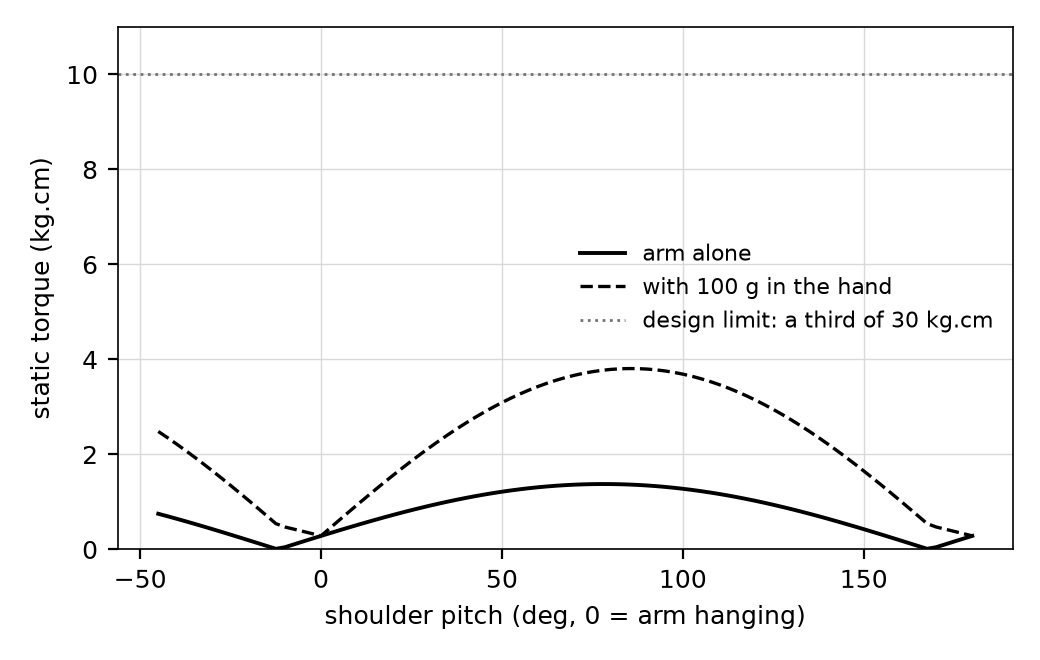
\includegraphics[width=0.49\linewidth]{figs/v2_shoulder_torque.png}\hfill
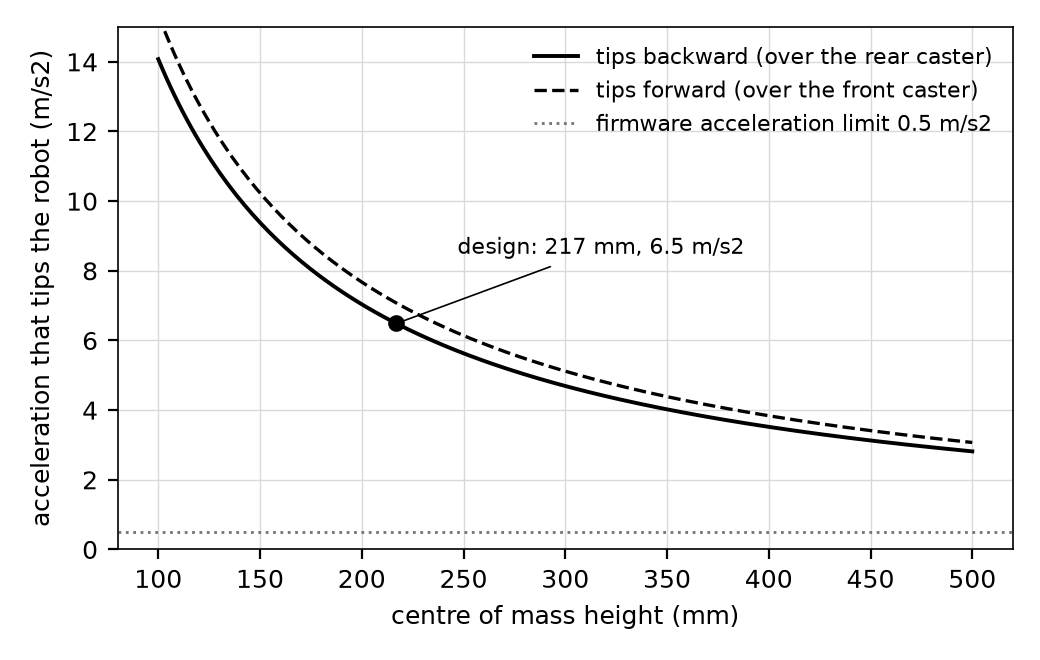
\includegraphics[width=0.49\linewidth]{figs/v2_tipover.png}
\caption{Left: static shoulder pitch torque over the whole range, computed by the twin, with and without 100\,g in the hand, against the design limit of a third of the rating. Right: acceleration that tips the robot against the height of the centre of mass; the design point is 13 times above the firmware limit.}
\end{figure}

\subsection{Motion: the firmware driving the full robot in MuJoCo}
The twin (\file{sim/generate_twin.py}) is built from the CAD meshes: joint axes measured from the servo horns, part masses from volume and density, kit components at their placed positions. \file{sim/firmware_sim.py} compiles the same controller that runs on the Mega and calls it every 10\,ms, exactly as \file{main.cpp} does on the robot, while the script plays the hardware:
\begin{itemize}
\item encoders: wheel angles turned into counts (1320 per turn);
\item range sensors: rangefinder rays turned into ToF readings (every 33\,ms, $\pm$5\,mm noise, 1.2\,m range) and ultrasonic readings (alternating every 60\,ms, $\pm$10\,mm, 1\,m);
\item gyro: the IMU site; motors: a DC-motor torque-speed line (10\,\kgcm{} stall, 200\,rpm no-load); servos: limited to their kit rating, limp without pulses.
\end{itemize}
It runs the minimum demonstration with the \texttt{DEMO} command: servos on, drive 1\,m, reverse 30\,cm, turn 90\deg, drive at a wall, wave, nod, shake, rest.

\begin{figure}[H]\centering
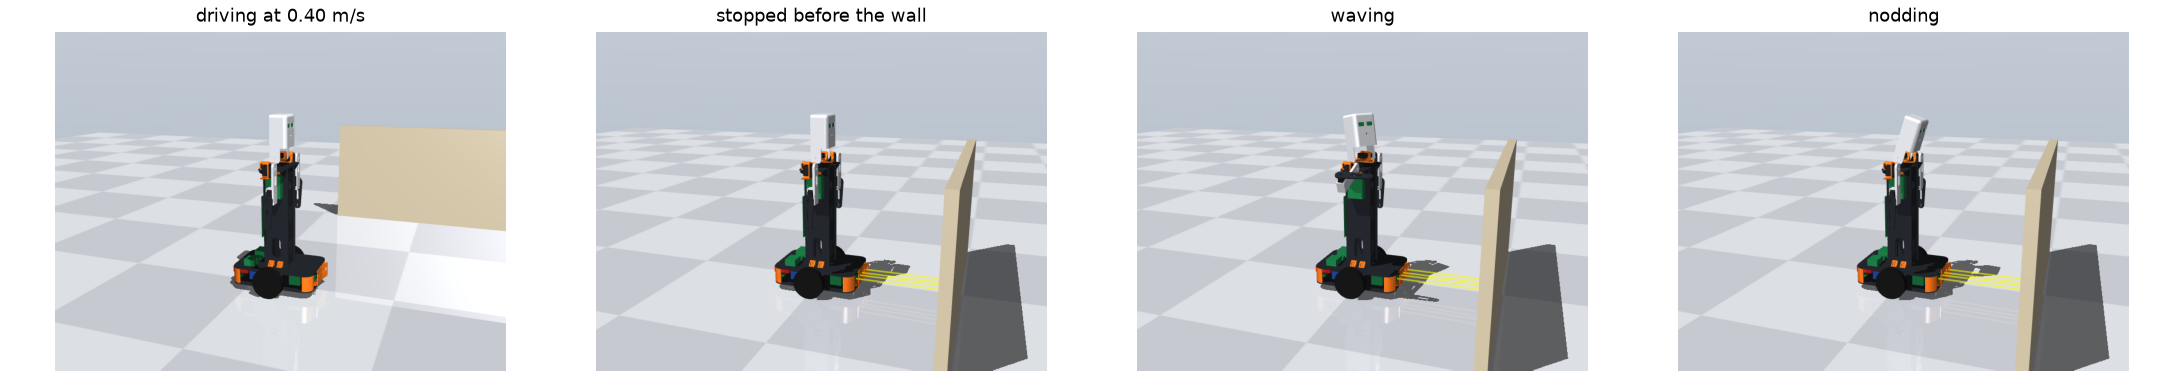
\includegraphics[width=\linewidth]{figs/v2_demo_frames.png}
\caption{Frames of the simulated demonstration: driving at 0.40\,m/s, stopped before the wall (the four range rays in yellow), waving, nodding.}
\end{figure}

\begin{table}[H]\small
\begin{tabularx}{\linewidth}{@{}P{44mm}LP{40mm}@{}}
\toprule
\textbf{Test} & \textbf{Simulated result} & \textbf{Pass criterion}\\
\midrule
T1 Straight drive, \texttt{FWD 100} & 0.998\,m true, drift 1\,mm & Error under 5\,cm\\
T1 Reverse, \texttt{BACK 30} & 0.299\,m & Error under 5\,cm\\
T2 Turn, \texttt{TURN 90} & 89.1\deg{} true (encoders 90.3\deg, gyro 89.1\deg), centre moved 0.8\,mm & Error under 5\deg\\
T3 Obstacle stop from 0.40\,m/s & Braking from 544\,mm, stops \textbf{378\,mm} from the wall, braking distance 150\,mm, tilt 0.6\deg & Stops at 300\,mm or more\\
T4 Wave & Peak 2.1\,\kgcm{} on the shoulder roll (7\,\% of rating), 1.5\,\kgcm{} on the elbow (8\,\%) & Under a third of rating\\
T5 Nod, shake & Head tilt 1.9\,\kgcm{} (15\,\%), head pan 1.3\,\kgcm{} (10\,\%) & Under a third of rating\\
T6 Whole \texttt{DEMO} & Completes in 29.9\,s; body tilt never above 0.64\deg; wheel torque peak 18\,\% of rated & Runs to the end\\
\bottomrule
\end{tabularx}
\end{table}

\begin{figure}[H]\centering
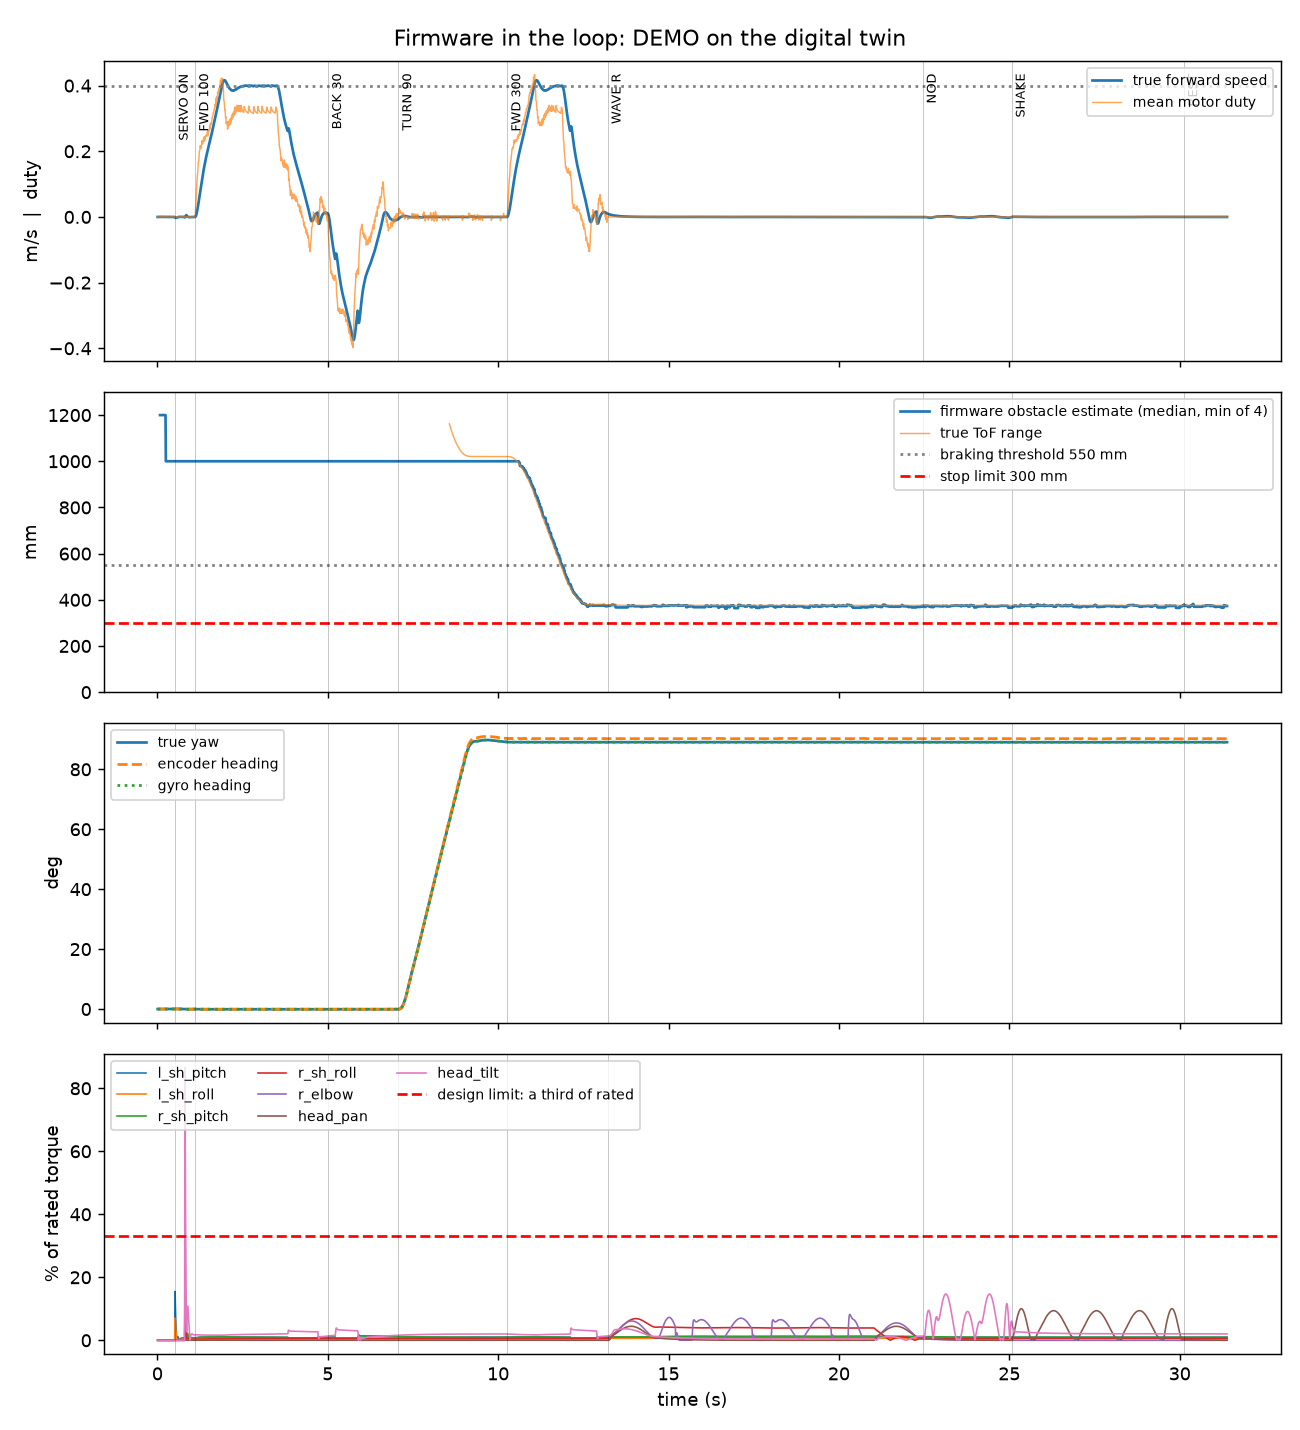
\includegraphics[width=0.80\linewidth]{figs/v2_demo_signals.png}
\caption{Signals over the simulated run: speed and motor duty; the firmware's obstacle estimate against the true range, with the 550\,mm braking threshold and the 300\,mm limit; heading from the encoders, the gyro and the truth; servo torques as a share of their rating.}
\end{figure}

\textbf{What the physics simulation showed that the hand calculations and the unit tests did not.}
\begin{itemize}
\item \textbf{Position tracking had to be added.} With speed loops only, the twin, with its real 4.8\,kg and a DC-motor torque curve, overshot \texttt{FWD 100} by 5\,cm and \texttt{TURN 90} by 10\deg. The unit tests had used a faster ideal motor and missed it. Making each wheel track the integral of its speed profile brought the errors to 2\,mm and 0.9\deg, and a test now checks motor time constants from 0.1 to 0.35\,s.
\item \textbf{The turn comes out 0.9\deg{} short} and the encoders read 1.2\deg{} more than the true yaw: the wide tyres make the effective track slightly larger than 300\,mm. The track is calibrated on the floor with \texttt{TURN 360}.
\item \textbf{Power-on snap.} The servos are limp until \texttt{SERVO ON}, so the head and arms sag; when the pulses start, the head tilt servo pulls back at up to 11\,\kgcm{} (87\,\% of its rating) for a fraction of a second. It is now a tracked risk: power the servos with the arms hanging and the head level.
\item \textbf{The robot rocks 0.6\deg{} onto its front caster when braking}, as computed in section~\ref{sec:stab}. Harmless.
\end{itemize}

\subsection{Clearance through the joint ranges}\label{sec:clear}
\file{sim/clearance.py} intersects the exact CAD solids of each arm and of the head with every other part of the robot, at every pose of a sweep through the firmware joint ranges, and along the logged \texttt{DEMO} trajectory. Parts that touch at the CAD pose by design (servo horns on their brackets) keep that contact as a baseline; a pose interferes when the overlap grows by more than 5\,mm\textsuperscript{3}.
\begin{table}[H]\small
\begin{tabularx}{\linewidth}{@{}P{50mm}P{44mm}L@{}}
\toprule
\textbf{Sweep} & \textbf{Range, step} & \textbf{Result}\\
\midrule
Each arm: pitch $\times$ roll $\times$ elbow & $-45$ to 180\deg{} $\times$ $-30$ to 120\deg{} $\times$ 0 to 135\deg; 15\deg, elbow 45\deg & \textbf{Interference only at roll $-30$\deg}: the upper arm meets the shoulder plate, the chest plate or a board\\
Inward roll, 1\deg{} steps, every 5\deg{} of pitch & $-30$ to 0\deg & First interference at \textbf{$-21$\deg}, both arms\\
Head: pan $\times$ tilt & $-90$ to 90\deg{} $\times$ $-30$ to 30\deg & Clear\\
Whole robot along the \texttt{DEMO} & 314 poses & Clear\\
\bottomrule
\end{tabularx}
\end{table}
\textbf{Design decision from this check.} The firmware stops inward shoulder roll at $-15$\deg{} at every pitch, 6\deg{} before contact. The rule inherited from an earlier version of the design (limit only while the arm hangs) left 8 interfering poses per arm on this design. No gesture uses inward roll, so nothing is lost. Cables are not modelled.
\begin{figure}[H]\centering
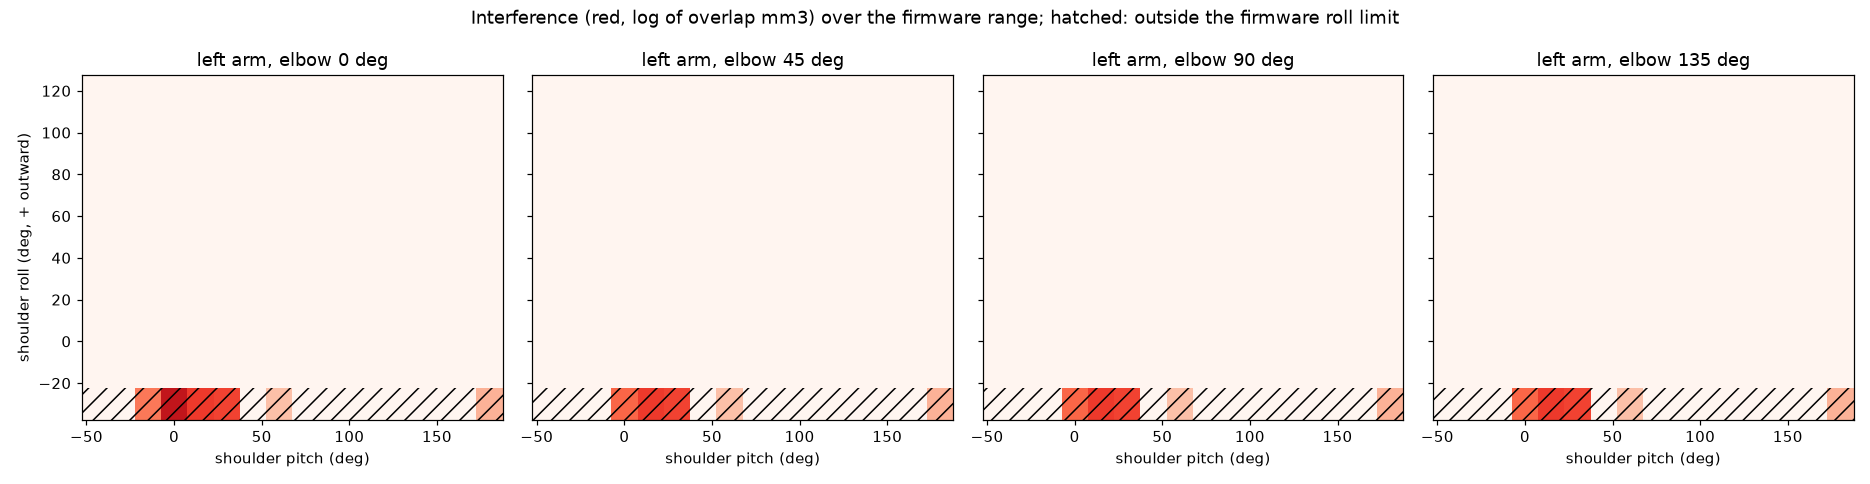
\includegraphics[width=\linewidth]{figs/v2_clearance_map.png}
\caption{Interference of the left arm over the firmware range, for four elbow angles. Hatched: outside the roll limit. Every red cell lies in the hatched band.}
\end{figure}

% =============================================================== 5 code
\clearpage
\section{Code}\label{sec:code}
Repository: \url{\repo}. The README gives the overview, architecture, wiring and pinout, and how to build and run each part; the commands below are the short version.

\subsection{Structure}
\begin{table}[H]\small
\begin{tabularx}{\linewidth}{@{}P{38mm}L@{}}
\toprule
\textbf{Folder} & \textbf{Content}\\
\midrule
\file{firmware/} & PlatformIO project for the Arduino Mega (C++). \file{lib/robot_core/}: the controller, with no Arduino code (\file{drive}, \file{obstacle}, \file{gestures}, \file{robot_core}: parser, state machine, safety, \texttt{DEMO}). \file{src/main.cpp}: hardware layer. \file{test/}: 30 unit tests. \file{protocol.md}: every command and message\\
\file{pi/} & Python service for the Pi 5: \file{link.py}, \file{behaviour.py}, \file{eyes.py}, \file{camera.py}, \file{web.py}; setup script and systemd unit\\
\file{sim/} & Twin generator, firmware-in-the-loop simulation, clearance check, results\\
\file{fabrication/} & Numbered print and cut files and their generator\\
\file{wiring/}, \file{info/}, \file{step_parts/} & Wiring diagram, drawings, STEP files\\
\bottomrule
\end{tabularx}
\end{table}
The build uses 3.2\,KB of the Mega's 8\,KB of RAM and 37\,KB of flash.

\subsection{Firmware loop and algorithms}
Every 10\,ms \file{main.cpp} reads the encoder counts (interrupts, 4$\times$ quadrature), any new ToF reading (non-blocking), one ultrasonic sensor every 60\,ms, the gyro rate, the battery voltage and the optional E-stop contact, calls the controller once, and writes the motor drivers (PWM at 3.9\,kHz) and, every other step, the servo channels that changed.
\begin{itemize}
\item \textbf{Motion profile.} The speed reference is ramped at 0.5\,m/s\textsuperscript{2} and capped at 0.40\,m/s (0.12\,m/s per wheel in turns); braking follows $v=\sqrt{2\cdot 0.8\,a\,d}$ so that each move ends on its target.
\item \textbf{Position tracking.} Each wheel follows the integral of the profile through a correction of 4\,(m/s)/m, then a PI speed loop with feed-forward on speed and on (filtered) acceleration. Straight lines stay straight because both wheels track the same position reference.
\item \textbf{Odometry and slip.} Encoder odometry; the gyro heading is integrated alongside and a disagreement above 10\deg{} after a turn is reported (\texttt{EVT SLIP}).
\item \textbf{Obstacle stop.} Median of the last three readings per sensor, then the minimum over the four sensors. Below 55\,cm, forward motion brakes at 0.5\,m/s\textsuperscript{2} and stays blocked until the path is clear above 65\,cm; reversing and turning stay allowed. If no sensor has reported for 0.5\,s, forward motion is refused.
\item \textbf{Gestures.} Keyframes in joint space played with a minimum-jerk profile $s(u)=10u^3-15u^4+6u^5$, timed so the peak speed is 90\deg/s; joint limits (section~\ref{sec:clear}) applied to every interpolated point.
\item \textbf{Safety.} Drivers disabled and servos released on emergency stop (latched until \texttt{RESET}), after 2\,s below 9.9\,V, or 0.5\,s after the last teleop command. Servo strips start 300\,ms apart.
\end{itemize}
Libraries: \texttt{Adafruit PWM Servo Driver} (PCA9685), \texttt{VL53L0X} (Pololu), \texttt{Wire}; encoders, ultrasonic sensors and IMU use short code of our own to keep the loop time fixed. On the Pi: \texttt{pyserial}, \texttt{Flask}, \texttt{Pillow}, \texttt{luma.oled}, \texttt{picamera2}.

\subsection{Serial protocol}
Text lines at 115200 baud, the same whether typed by a person, sent by the Pi or sent by the simulator. Each command answers \texttt{OK}, then \texttt{DONE <cmd> ok|blocked|stopped} when it finishes, or \texttt{ERR} with a reason.
\begin{table}[H]\small
\begin{tabularx}{\linewidth}{@{}P{62mm}L@{}}
\toprule
\textbf{Command} & \textbf{Effect}\\
\midrule
\texttt{FWD <cm>}, \texttt{BACK <cm>} & Drive a distance at the capped speed\\
\texttt{TURN <deg>} & Turn on the spot, positive is left\\
\texttt{VEL <mm/s> <deg/s>} & Teleop; must be repeated within 0.5\,s\\
\texttt{STOP} & Ramp to zero, freeze the servos, abort the demonstration\\
\texttt{ARM L|R <pitch> <roll> <elbow>}, \texttt{HEAD <pan> <tilt>} & Move to joint angles\\
\texttt{WAVE [L|R]}, \texttt{POINT [L|R]}, \texttt{NOD}, \texttt{SHAKE}, \texttt{REST} & Stored gestures\\
\texttt{SERVO ON|OFF}, \texttt{RESET} & Servo power, clear a fault\\
\texttt{DEMO} & The full minimum demonstration\\
\texttt{STATE?}, \texttt{STREAM <hz>} & State: mode, faults, pose, speed, obstacle, battery, running command\\
\texttt{CAL ENC|MOTOR|PULSE|INFO} & Bench calibration (robot only, not reachable from the web page)\\
\bottomrule
\end{tabularx}
\end{table}
Events: \texttt{EVT BLOCKED}, \texttt{CLEAR}, \texttt{NO\_RANGE}, \texttt{FAULT ESTOP|LOWBAT}, \texttt{VBAT\_LOW}, \texttt{SLIP}, \texttt{VEL\_TIMEOUT}, \texttt{DEMO <step>}.

\subsection{Raspberry Pi service}
\file{link.py} owns the serial port and reconnects on its own; \file{behaviour.py} gives the robot its character from the Mega's events (surprised eyes when blocked, happy on a wave, eyes that look toward a turn, sleepy when idle) and takes no safety decision; \file{eyes.py} draws the two OLEDs; \file{camera.py} streams the head camera; \file{web.py} serves the control page (STOP, hold-to-drive, moves, gestures, \texttt{DEMO}, live state, eyes, camera stream) and forwards only commands from a whitelist. The link also opens a TCP address, so the whole Pi service runs on a laptop against the simulator.

\subsection{Build and run}
{\small
\begin{tabularx}{\linewidth}{@{}P{58mm}L@{}}
Unit tests of the controller & \file{make -C firmware test}\\
Build and flash the Mega & \file{pio run -t upload} (in \file{firmware/})\\
Firmware on the twin, DEMO & \file{python sim/firmware_sim.py}\\
Clearance check & \file{python sim/clearance.py}\\
Pi service on the robot & \file{python -m humanoid_pi} (in \file{pi/})\\
Pi service against the twin & \file{python sim/firmware_sim.py --tcp 5555}, then \file{python -m humanoid_pi --port socket://localhost:5555}\\
\end{tabularx}}

\end{document}
